\makeatletter
\newcommand{\rome}[1]{\romannumeral #1}
\newcommand{\Rome}[1]{\expandafter\@slowromancap\romannumeral #1@}
\newcommand{\bsy}[1]{\boldsymbol{{}#1}}
\makeatother
\title{Elastic wave-equation-based reflection kernel analysis and traveltime inversion using wave mode decomposition}
\author{
	Tengfei Wang\footnotemark[1], Jiubing Cheng\footnotemark[2], Qiang Guo\footnotemark[3] and Chenlong Wang\footnotemark[4] 
}
\address{
	\footnotemark[1] School of Ocean and Earth Science, Tongji University, Shanghai,
	China. E-mail: 1110701@tongji.edu.cn\\
	\footnotemark[2] State Key Laboratory of Marine Geology, Tongji University,
	Shanghai, China. E-mail: cjb1206@tongji.edu.cn\\
	\footnotemark[3] School of Ocean and Earth Science, Tongji University, Shanghai,
	China. E-mail: 1110701@tongji.edu.cn\\
	\footnotemark[4] State Key Laboratory of Marine Geology, Tongji University,
	Shanghai, China. E-mail: cjb1206@tongji.edu.cn
}
\lefthead{Wang et al.}
\righthead{Elastic reflection kernel analysis and traveltime inversion}
\maketitle

\begin{abstract}
%Elastic full waveform inversion (EFWI) provides high-resolution parameter estimation of the
%subsurface but requires good initial guess of the true model.
Elastic reflection waveform inversion (ERWI) utilize the reflections to update the low and
intermediate wavenumber in the deeper part of elastic model, which can provide good initial models
for elastic full waveform inversion (EFWI). Though ERWI can mitigate the nonlinearity to some
extent, it is still stuck with the cycle-skipping problem due to the objective function of waveform fitting. 
%the cycle-skipping of traveltime
%objective function will be less severe
%compared with the previous one. 
%Therefore, 
Building initial P and S wave velocity models for EFWI through elastic wave-equation
reflections traveltime inversion (ERTI) would be effective and robust
since traveltime information relates to the background model more linearly. 
The wave mode decomposition, both on the recording surface and in the underground space, are important for ERTI.
On the one hand,
P/S separation of multicomponent seismograms on the surface provides 
individual P or S wave data residuals.
Thus, we implement the ERTI using the $L_2$ norm of the isolated P or S wave traveltime
residuals extracted by the dynamic image warping (DIW) as objective function.
On the other hand, the underground spatial wave mode decomposition provides separated wavefields to precondition
the kernels or gradients.
However, the reflection kernels in elastic media are complicated and difficult to use, especially when
calculating the gradient of S-wave
velocity. The investigation of reflection kernels show that mode decomposition can suppress the artifacts in
gradient calculation. 
%Besides, the model regularization through local dip-dependent smooth filter ensures the inversion converging to a
%geological model. 
Accordingly, a two-step inversion strategy is adopted to effectively reduce the nonlinearity of inversion, in which PP reflections are first used to invert $V_p$,
followed by $V_s$ inversion with PS reflections based on the well recovered $V_p$. 
%To avoid the mismeasurement of PS traveltime residual, the well recovered PP image are used to
%generate the PS reflections. 
%Through the layer stripping strategy, we rebuild the background elastic
%model from shallow the deep.
%P/S separation of multicomponent seismograms  spatial wave mode
%decomposition provides P or S wavefields, which help
%to  reduce the nonlinearty of inversion effectively.
%The kernel of reflection wavepath proves that mode decomposition can surpress the artifacts in
%the reflection inversion. 
Numerical example of Sigsbee2A model validates the effectiveness of the
algorithms and strategies for ERTI.
%Synthetic example on the Sigbee2A model proves the validity
%of our method for recovering the long wavelength components of the model.
%Numerical example of Sigsbee2A model validates the effectivenss of the 
%algorithms and strategies for EWERTI, whose results also are tested through EFWI.
\end{abstract}
\section{Introduction}
With the emergence of long-offset wide-azimuth acquisitions and broad-band sources,
full waveform inversion (FWI) has been recognized as an
efficient tool for constructing velocity models and quantitative seismic imaging, see
\cite{virieux2009overview} for a review.
Though the acoustic FWI, primarily focusing on P-wave velocity inversion, has been
widely studied in the past decades
\cite[]{tarantola1984,pratt1998gauss,shipp:2002}, people are paying more attention
to the waveform inversion under the elastic assumption, referred to as elastic full waveform inversion
(EFWI) \cite[]{tarantola1986}.
Waveform inversion provides high-resolution model estimation of the elastic
properties, but it
suffers from the cycle-skipping easily because of its insensitivity to the low and intermediate wavenumber components of the model
when the acquisition illumination is poor and/or good initial models are unavailable during the inversion\cite[]{sears2008,brossier2009}. 
Besides, multi-parameter trade-off effects and more complicated elastic wave phenomena 
will further increase the difficulties for EFWI.
To deal with the nonlinearities and parameter trade-offs, more
preconditioning, hierarchical strategies and parameterization investigation should be
considered during EFWI 
\cite[]{sears2008,prieux:2013b,operto2013guided,wang:2015,Oh2016}.

%In the surface observation geometry, full waveform inversion (FWI) often suffers from the
%local minimal due to the absence of low frequencies in the data when the low-wavenumber
%component is missing in the initial model.
For the classical FWI, the long-offset data
corresponding to diving waves are very important to build the long-to-intermediate
wavelengths of the model. However, the penetration depths of
diving waves are always far from sufficient to reach the target in the deeper part
%with the limited surface offset,
even using the wide-aperture surveys. 
In addition, the low signal-to-noise ratio at the far
offset is also a limit for the classical FWI relying on the diving waves. 
Therefore, people tried to utilize the reflections
to help build the macro-model containing low-to-intermediate wavenumber
in the deep part\cite[]{Stork1992,ChaventEtAl1994,clement:2001,Symes2008a,xu:2012}.
This process can be implemented in the image domain or the data domain. 
Actually, the image-domain ray-based tomography
\cite[]{Stork1992,Woodward1992,Woodward2008,Jones2010} has already been a standard workflow to obtain the background velocity by flatting the common
image gathers. But when the lateral velocity variation is strong, the ray-based method would fail to
present the wave propagation underground.
%, which will probably lead to the failure of tomography.  
To overcome the limit of ray theory, 
people have made great efforts to develop the approaches of reflection inversion that employ
waveform or traveltime information based on wave-equation
\cite[]{xu:2012,Ma2013,Wu2015b,Zhou2015,Wang2015,Chi2015}.

The misfit function of reflection inversion can be built in image domain in the manner of wave equation migration
velocity analysis (WEMVA), which tries to maximize the
energy at zero-offset location in the extended subsurface image gathers
\cite[]{Symes2008,Almomin2012,SunEtAl2012,biondi2013}.
%Alternatively, the image domain strategy also can be fulfilled by the wave equation
%migration velocity analysis (WEMVA), in which velocity is updated
%through minimizing the energy of non-zero offset on the extended-domain gathers \cite[]{Symes, 2008; Fleury
%and Perrone, 2012; Biondi and Almomin, 2013}.
\cite{RaknesEtAl2016} 
developed an image-domain method to invert P-wave velocity ($V_p$) in the 3D elastic media. 
\cite{Wang2017WEMVA} proposed to employ the extended PS image in WEMVA to update the
S-wave velocity ($V_s$) with the help of elastic wave mode decomposition.
%But it is a big issue that the extended domain approach requires huge computational cost,
%especially in 3D case.
However, the extended-domain methods are limited in filed data due to its prohibitively computational cost,
especially in 3D case.
While in the data domain,
\cite{xu:2012} suggested using a reflection waveform inversion (RWI) method to suppress the
nonlinearity in FWI, 
which aim to invert the long-wavelength components of the model by using the reflections 
predicted by migration/demigration process.
Recently, \cite{Zhou2015} proposed a joint FWI method that combines the diving and reflected waves to
utilize both RWI and the conventional FWI.
\cite{Wu2015b} developed an RWI scheme to simultaneously invert the background velocity and the
perturbation in acoustic media,  and recently extended to elastic case by
\cite{Guo2016}.
RWI highly relies on the accurate reflectivity to generate the reflections that can match the
observed data. However, it is very challenging and also expensive to obtain a good reflectivity model through 
least-square migration when initial model is far away from the true one.

%In addition, \cite{Wang:2015} found that wave mode decomposition may be beneficial to deal with the
%elastic parameter trade-offs.
Compared with the waveform information, 
%traveltime is more sensitive and linearly related to
%low-wavenumber model perturbation. Using traveltime inversion will be more robust and helpful to
%build appropriate initial models containing long-wavelength components for
%conventional FWI \cite[]{Ma2013, Wang2015,Chi2015, Luo2016}.
traveltime is more sensitive and linearly related to
the low-wavenumber components of the model. Therefore, traveltime inversion will be more robust and helpful to
build good initial models for conventional FWI
\cite[]{WangEtAl2014}.
\cite{Ma2013} introduced a wave equation reflected traveltime inversion method
based on dynamic image warping (DIW) to build the low wavenumber of the model. 
\cite{Chi2015} and \cite{Wang2015} employed correlation-based method to extract the
temporal or spatial lag to implement the reflection inversion. 
Elastic reflections carry the background information of the P and S wave velocities, 
which can help to rebuild the good initial velocity models for EFWI.
Unfortunately, in elastic case, traveltime shifts of a particular wave mode are difficult
to extract due to the complicated wave phenomenons, such as mode-conversions.
%It is common to observe that different mode-conversions, mainly P-P
%and P-S events, overlap and intersect with each other. The cross points between events
%would be singularities for traveltime difference estimation even using the local shift estimation 
%method like DIW.
Therefore, the estimated time shifts would be inaccurate if using the
original multicomponent seismograms directly.
%, which makes the elastic wave-equation reflection
%traveltime inversion (ERTI) difficult to implement.
In addition, since the multi-parameter trade-offs will increase the
nonlinearity of inversion, more hierarchical strategies should be considered to deal
with this problem.
\cite{WangEtAl2017} 
preconditioned the gradients of EFWI through wave mode decomposition to mitigate
parameter trade-offs and explained that this precondition partially utilize the off-diagonal Hessian blocks
when inverting $V_s$.  
As a natural tool to obtain the separated data subsets, the wave mode decomposition similarly
has the potential to precondition the elastic wave-equation reflection traveltime
inversion (ERTI) with more flexible hierarchical strategies.

%In this paper,
%we aim to tackle the traveltime misfits of P-P and P-S reflections with the help
%of wave mode decomposition and dynamic image warping (DIW) \cite[]{Hale2013}.
%Then, we use the traveltime of P-P and P-S reflections to implement the 
%WERTI method \cite[]{Ma2013} with a two-stage workflow.
%Finally, the numerical example of Sigsee2A model proves the robustness and validity of our
%elastic WERTI method.


%The key point of RWI is to project the data-domain residuals back to the reflection wavepath to 
%is to project the data-domain residuals back to the reflection wavepath to 

%for both the imaging condition and the forward modelling in each iteration.

%\cite{Zhou2015} proposed a joint FWI method to combine the diving and reflected waves to
%utilize both the conventional FWI and RWI.
%In addition, \cite{Wang:2015} found that wave mode decomposition may be beneficial to deal with the
%elastic parameter trade-offs.
%build appropriate initial models containing long-wavelength components for
%Unfortunately, in elastic case, traveltimes of a particular wave mode are difficult
%to extract due to the complicated mode-conversions. 

In this paper,   
we will exploit the traveltime misfits of PP and PS reflections to implement the ERTI
approach with the aid
of wave mode decomposition and DIW \cite[]{Hale2013}.
%In this abstract, we separate the PP and PS reflections in the observed and predicted multicomponent data to
%extract the individual traveltime residuals through DIW \cite[]{Hale2013}.
%using surface P/S wave
%separation. Dynamic image warping \cite[]{Hale2013} helps to extract the local traveltime residual
%between the observed and the predicted data.
First, 
the elastic reflection kernel and its components of different wave modes are
calculated and the implications to suppress the artifacts in the gradient calculation
are investigated.
%to investigate  the effectiveness of mode decomposition on suppressing the artifacts in the gradient calculation.
Then, P/S separation of multicomponent seismograms is applied to the observed and predicted reflection data 
to extract the individual traveltime residuals of PP and PS reflections through DIW. 
Based on the analysis of elastic reflection kernels and the separated traveltime residuals, 
we design a two-stage workflow to implement
the ERTI method,
in which the traveltime of PP reflections are firstly used to recover the background
$V_p$ model and then the traveltime of PS reflections are used to recover the background $V_s$ model
.
According to our investigation, it is quite difficult to estimate the time shifts of PS reflections if we
use the PS image to predict the corresponding reflection using demigration.
%During the $V_s$ inversion, the PS reflections are predicted by the PP image to avoid
%the wrongly estimated time shifts when using PS image.
Moreover, we precondition the $V_s$ gradient through the spatial wave mode
decomposition.
Finally, the numerical example of Sigsee2A model proves the robustness and validity of our
ERTI method.

\section{Theory of ERTI}
rssume that there is a perturbation $\delta c_{ijkl}$ in the background elastic media
$c_{ijkl}$, the background wavefileds $u_i$ and perturbed wavefields
$\delta u_i$ satisfy:
\begin{equation}
    \rho \frac{\partial u^2_i}{\partial t^2}  -
    \frac{\partial}{\partial x_j}\left[ 
        c_{ijkl}\frac{\partial u_{k}}{\partial
        x_l}\right]=f_i,
    \label{eq:WE} 
\end{equation}
and
\begin{equation}
    \rho \frac{\partial \delta u^2_i}{\partial t^2}  -
    \frac{\partial}{\partial x_j}\left[ 
        c_{ijkl}\frac{\partial \delta u_{k}}{\partial
        x_l}\right]=\frac{\partial}{\partial x_j}\left[\delta c_{ijkl}\frac{\partial u_{k}}{\partial x_l}\right],
    \label{eq:DeltaWE} 
\end{equation}
in the sense of first-order elastic scattering, where $\delta u_i$ can be seen as the demigrated reflection data using the image
perturbation $\delta c_{ijkl}$ obtained from RTM or other imaging method. In ERTI, we
aim to minimize the traveltime differences between observed data
$\mathbf{d}^{o}$ and
calculated data $\mathbf{d}^{c}$, then
the objective function can be expressed as:
%\begin{equation}
%	E=\frac{1}{2}\int\tau^2(\mathbf{x_r},t;\mathbf{x_s})dtd\mathbf{x_r}d\mathbf{x_s},
%    \label{eq:Objectivefunction} 
%\end{equation}
\begin{equation}
	\left\{
		\begin{aligned}
			&\tau(\mathbf{x_r},t;\mathbf{x_s})=\mathop{\arg\min}_{\tau}
			\parallel\mathbf{d}^{c}(\mathbf{x}_r,t;\mathbf{x}_s)-\mathbf{d}^{o}(\mathbf{x}_r,t+\tau;\mathbf{x}_s)\parallel^2\\
    &E=\frac{1}{2}\int\tau^2(\mathbf{x_r},t;\mathbf{x_s})dtd\mathbf{x_r}d\mathbf{x_s},
		\end{aligned}
	\right.
    \label{eq:Objectivefunction} 
\end{equation}
where the time differences $\tau(\mathbf{x_r},t;\mathbf{x_s})$ can be extracted
through DIW (The readers can refer to \cite{Hale2013} for detail).
After a similar derivation as in \cite{Ma2013} (see Appendix A ), the gradients of equation \eqref{eq:Objectivefunction} can be expressed as:
\begin{equation}
	\frac{\partial E}{\partial c_{ijkl}}=-\int (\frac{\partial u_{i}}{\partial
	x_j}\frac{\partial \delta \psi_{k}}{\partial x_l}+\frac{\partial \delta u_{i}}{\partial
	x_j}\frac{\partial \psi_{k}}{\partial x_l}),
    \label{eq:GradientCijkl}
\end{equation}
where $u_i$ and $\delta u_i$ are the state variables, while $\psi_i$ and $\delta
\psi_i$ are the adjoint state variables satisfying:
\begin{equation}
    \rho \frac{\partial \psi^2_i}{\partial t^2}  -
    \frac{\partial}{\partial x_j}\left[ 
        c_{ijkl}\frac{\partial \psi_{k}}{\partial
		x_l}\right]=\tau(\mathbf{x_r},t;\mathbf{x_s})\frac{\dot{d}^o_i(\mathbf{x_r},t+\tau;\mathbf{x_s})}{h_i(\mathbf{x_r},t;\mathbf{x_s})},
    \label{eq:AdjointWE} 
\end{equation}
and
\begin{equation}
    \rho \frac{\partial \delta \psi^2_i}{\partial t^2}  -
    \frac{\partial}{\partial x_j}\left[ 
        c_{ijkl}\frac{\partial \delta \psi_{k}}{\partial
        x_l}\right]=\frac{\partial}{\partial x_j}\left[\delta c_{ijkl}\frac{\partial
		\psi_{k}}{\partial x_l}\right],
    \label{eq:AdjointDeltaWE} 
\end{equation}
with
$h_i(\mathbf{x_r},t)=\dot{d}^o_i(\mathbf{x_r},t+\tau)^2-\ddot{d}^o_i(\mathbf{x_r},t+\tau)(d^c_i(\mathbf{x_r},t)-d^o_i(\mathbf{x_r},t+\tau)$.
(The hat dot denotes the time derivative.) On the right-hand-side (RHS) of equation
\eqref{eq:GradientCijkl}, the two terms indicate the source and receiver
parts of the reflection wavepath, respectively. For simplicity, we derive the
gradients of stiffness
coefficients for inversion. But the velocity parameterization will be more reasonable
to implement the traveltime inversion.
Thus, we can get the gradients in terms of P- and S- wave velocities through the chain rule:
\begin{equation}
	\begin{split}
	&\frac{\partial E}{\partial V_p}=2\rho V_p\frac{\partial E}{\partial
		c_{ijkl}}\delta_{ij}\delta_{kl}, \\
	&\frac{\partial E}{\partial V_s}=2\rho V_s\frac{\partial
	E}{\partial c_{ijkl}}(-2\delta_{ij}\delta_{kl}+\delta_{ik}\delta_{jl}+
	\delta_{il}\delta_{jk}).
	\end{split}
    \label{eq:GradientVel}
\end{equation}

\section{Elastic Born reflection kernels}
Reflection traveltime and waveform inversions utilize different objective functions
but share the same reflection wavepath information (reflection kernels). 
%From the perspective of gradient calculation, different objective functions only induce different types of adjoint
%sources. 
Therefore, the key point of reflection inversion is how to calculate and utilize the reflection kernel. 
%Different types of objective funtion only induce different types of adjoint sources.
In elastic case, due to the complex wave phenomenons, the cross-correlations between
different wave mode conversions will generates cross-talks in the kernel. Therefore, the wavepath of elastic reflections will 
be far more complicated than that in acoustic case \cite[]{Wang2017}.
For simplicity, we rewrite \eqref{eq:GradientCijkl} as follow:
\begin{equation}
    \nabla E(
    \mathbf{m}_0)=-\int(
    \mathbf{u}\cdot\delta \boldsymbol{\psi}
    +\delta
    \mathbf{u}\cdot{\boldsymbol{\psi}})
    \label{eq:kernelgradient} 
\end{equation} 
with $\mathbf{m}_0$ is the background model, $\mathbf{u}$ and $\boldsymbol{\psi}$ are the forward and adjoint background wavefields,
$\delta\mathbf{u}$ and $\delta \boldsymbol{\psi}$ are the forward and adjoint perturbed wavefields.
The operator $\cdot$ denotes the cross correlation between two wavefields. 
Note that, equation \eqref{eq:kernelgradient} just schematically shows the manner of cross correlation. 
The detailed formulas should be derived according to the parameterization through
chain rule as in equation \eqref{eq:GradientVel}.

Since in the elastic case, the four wavefields in eq. \eqref{kernelgradient} contain both P and S
waves, the cross-correlation between different wave modes may cause interference to
gradients \cite[]{Wang2017}.
To analyze the elastic reflection kernels, 
we decompose the original kernel into four components which 
correspond to the cross-correlation of different wave modes, respectively, as follows:
%Tthe above formula can be decomposed into four types with:
\begin{equation}
    K_{m_0}^{MN}     
    =-\int(\mathbf{u}^M\cdot\delta \boldsymbol{\psi}^N
    +\delta  \mathbf{u}^M\cdot\boldsymbol{\psi}^N),\\
    \label{eq:decompkernel} 
\end{equation}
where $M,N\in\{P,S\}$.
$K_{m_0}^{MN}$ represents the cross correlation between the $M$ mode forward wavefields and the 
$N$ mode adjoint wavefields. 
As illustrated in {\color{red}Fig. \ref{fig:11}}, this
kernel can be considered as the cross-correlation between the forward wavefields
emitted from a virtual source at a mirror location and the adjoint wavefields
back-propagated from the receiver. If the traveltime of the adjoint wavefields (injected at
receiver) approximately equals to the forward wavefields, the cross-correlation will
produce the low-frequency wavepath information. Otherwise, the cross-correlation
should be a high-wavenumber migration impulse. For example, $K^{PS}$ is the
cross-correlation of P-mode forward wavefield and S-mode adjoint wavefields, but has
little to do with the PS mode data.
%Note, it does not denote the kernel of $MN$ mode data. For example, the reflection 
%kernel of PS data should be $(\mathbf{u}^P\cdot\delta \boldsymbol{\psi}^P +\delta
%\mathbf{u}^S\cdot\boldsymbol{\psi}^S)$ but not $K^{PS}$.

Numerically, we calculate the kernels with the single-source-receiver data
which are synthesized for a single reflector with a pure P-wave source.
%Here we use a waveform data residual as the adjoint source for back-propagation.
Since different objective functions only induce different types of adjoint
sources from the perspective of gradient calculation, the investigation of kernels can
be done by using a waveform data residual as the adjoint source for back-propagation.
We use the $V_p$ - $V_s$ parameterization as in equation \eqref{eq:GradientVel}.
In the first test, we place a single $V_p$ reflector in the homogeneous background (Fig \ref{fig:kernel1_vp}a and b). 
%We use the single source-receiver reflection data to calculate the kernel.
Since there is no perturbation of $V_s$, only PP reflection exist in the data (almost
the same as in acoustic media), which means mode decomposition is unnecessary in this
case.
As shown in Figure \ref{fig:kernel1_vp}c and d, the reflection kernel consists of two ``rabbit-ear'', the
source and receiver parts. $K_{V_p}$ produces the low-wavenumber PP reflection
wavepath as expected.
While in $K_{V_s}$, the energy focus on the edge of the wavepath rather than the first Fresnel-Zone as in the $V_p$ kernel.
One plausible reason is that the $V_s$ kernel is relatively insensitive to the PP data generated by $V_p$ reflector.
Besides, we can see the migration impulse below the reflector due to the down-going perturbed wavefields
(Zone D mentioned by \cite{Zhou2015}).


In the second test, we use the $V_s$ reflector (Fig \ref{fig:kernel2}a and b) to generate both PP
and PS reflections.
%The $V_s$ reflector produces both PP and PS data. 
The $V_p$ kernel excludes S-wavefield automatically because of the divergence operator 
implied in the term $\delta_{ij}\delta_{kl}$ (see eq. \eqref{eq:GradientVel}). 
However, $\delta \boldsymbol{\psi}$ contains the converted SP wavefields 
induced by the back-propagated  $\boldsymbol{\psi}^S$ at the location of reflector.
These non-physical wavefields make the $V_p$ kernel slightly different from that in Figure \ref{fig:kernel1_vp}c.
To remove these non-physical artifacts in $K_{V_p}$, we should only inject the PP data during the
back-propagation. 
%If we only back-propagate the PP data, $V_p$ kernel will be the same as Figure \ref{fig:kernel1_vp}c.

For the $V_s$ kernel (Figure \ref{fig:kernel2}d), due to mode conversions, multi-wavepaths overlapping with each other 
make it much more difficult to find the correct reflection kernel. 
The straightforward utilization of this kernel in gradient calculation will very likely cause severe
cross-talk during reflection inversion.
According to equation
\eqref{eq:decompkernel}, we calculate the components of $K_{V_s}$, as shown in Figure
\ref{fig:kernel2_vs_decomp}. We observe that the $K^{PP}_{V_s}$ is similar to $K^{PP}_{V_p}$ but with an opposite
sign. This is because the term $\delta_{ij}\delta_{kl}$ implied divergence operator has
a negative sign in the $V_s$ gradient (eq. \eqref{eq:GradientVel}).
$K^{PS}_{V_s}$ and $K^{SP}_{V_s}$ mainly consist of high-wavenumber energy
corresponding to the migration impulse of cross-mode wavefields. Most importantly, 
we expect to update the $V_s$ model through the S-wavepath in PS reflection, which is
exactly the component $K^{SS}_{V_s}$.  Figure \ref{fig:kernel2_vs_decomp}d shows that the
separated S-wavepath of PS reflection is little affected by the P-wavefields. 
%S-wave part of the PS reflection wavepath. 
{\color{red}Therefore, we recommend using $K^{SS}_{V_s}$ to mitigate the cross-talks in $V_s$ gradient calculation.

To investigate the implication of the components of the kernel, }

\section{Workflow of elastic WERTI}
In elastic case, it is common to observe that different mode-conversions, mainly PP
and PS events, overlap and intersect with each other in the original multi-component
seismograms . The cross points between events
would be singularities for traveltime difference estimation through DIW.
%DIW extracts the reflection traveltime differences in data domain. In elastic case, %PP and PS reflections 
%the cross points between different mode-conversions would be singularities for DIW.
Therefore, the estimated $\tau(\mathbf{x_r},t;\mathbf{x_s})$ would be inaccurate due
to these singularities.
%if using the original multicomponent seismic data, which makes equation \eqref{eq:GradientVel} difficult to implement.
Besides, according to the reflection kernel analysis, individually injecting separated
PP or PS seismograms
can mitigate the cross-talk in gradient calculation. 
Thus, we decompose the observed and synthesized data into P- and S-wave
parts through P/S separation of multi-component seismograms \cite[]{Li2016a}.
In this way, the traveltime differences can be decoupled into PP and
PS parts by DIW. Accordingly, we implement the ERTI through a two-stage
workflow, i.e. estimating $V_p$ using PP reflections followed by the $V_s$ estimation
using PS reflections.

\subsection{Stage \uppercase\expandafter{\romannumeral1}: PP reflection for $V_p$}
In this stage, we use traveltimes of PP reflection to recover the low-to-intermediate wavenumbers of $V_p$ model. 
The perturbation of $V_p$ ($\delta V_p$) is obtained through elastic reverse time migration (ERTM). 
When the migration velocity model is inaccurate, 
%the migration/demigration of large-offset data would produce deviated
%zero-offset two-way travletime, which will increase the nonlinearity of inversion.
%Therefore, 
people always assume
the two way travletime of zero-offset as an invariants during reflection inversion, such as reflection traveltime tomography or RWI,
and thus use the zero or small offset data to generate the velocity perturbation \cite[]{Zhou2015}. 
Nonetheless, this method still may have problem to ensure a correct zero offset traveltime in the
demigration when velocity anomaly is complex. A better method would be the demigration with extended
image \cite[]{Webill2013, Symes2015, Qiang2017}, but it is out of the scope of this paper.
Besides, since the traveltime rather than the amplitude is fitted in ERTI, 
ERTM (instead of its least-squares counterpart) is sufficient to obtain the image perturbation for
the kinematic demigration.
%but not a least-squares manner (LSRTM) to find the correct reflectivity. 
Thus, the objective function can be written as:
\begin{equation}
	\left\{
		\begin{aligned}
			&\tau_{pp}(\mathbf{x_r},t;\mathbf{x_s})=\mathop{\arg\min}_{\tau}
			\parallel\mathbf{d}^{c}_{pp}(\mathbf{x}_r,t;\mathbf{x}_s)-\mathbf{d}^{o}_{pp}(\mathbf{x}_r,t+\tau;\mathbf{x}_s)\parallel^2\\
			&E_{pp}=\frac{1}{2}\int\tau^2_{pp}(\mathbf{x_r},t;\mathbf{x_s})dtd\mathbf{x_r}d\mathbf{x_s},
		\end{aligned}
	\right.
    \label{eq:ObjectivefunctionPP} 
\end{equation}
where $d^{c}_{pp}$ and $d^{o}_{pp}$ are synthesized and observed PP reflection through the P/S
separation on the recording surface, respectively. According to the previous derivation, we can
obtain the gradient of  $V_p$, i.e. $\frac{\partial E}{\partial
V_p}$.
Note that, 
the divergence operator is implied in $\frac{\partial
E}{\partial V_p}$, which makes the gradient calculation only involve PP reflection.
%is similar to the $V_p$ gradient of EFWI.
Therefore, the PP reflection traveltime inversion for $V_p$ in elastic media is similar to the acoustic case
except that we need the isolation of PS component in the former one. In addition, the separated
P-wave reflections may include some SP conversions due to the source-side effects in the elastic
case. This may lead to the mismatch of the traveltime inversion.
%calculate RHS of equation \eqref{eq:AdjointWE} and replacing $\delta c_{ijkl}$ with
%$\delta V_p$ in equation \eqref{eq:DeltaWE} and \eqref{eq:AdjointDeltaWE}.
\subsection{Stage \uppercase\expandafter{\romannumeral2}: PS reflection for $V_s$}
In the second stage, we utilize the PS reflections to retrieve the background component of
$V_s$ model. Similarly, the objective function becomes:
\begin{equation}
	\left\{
		\begin{aligned}
			&\tau_{ps}(\mathbf{x_r},t;\mathbf{x_s})=\mathop{\arg\min}_{\tau}
			\parallel\mathbf{d}^{c}_{ps}(\mathbf{x}_r,t;\mathbf{x}_s)-\mathbf{d}^{o}_{ps}(\mathbf{x}_r,t+\tau;\mathbf{x}_s)\parallel^2\\
			&E_{ps}=\frac{1}{2}\int\tau^2_{ps}(\mathbf{x_r},t;\mathbf{x_s})dtd\mathbf{x_r}d\mathbf{x_s}.
		\end{aligned}
	\right.
    \label{eq:ObjectivefunctionPP} 
\end{equation}
where $d^{c}_{ps}$ and $d^{o}_{ps}$ are synthesized and observed PS reflections, respectively.
After the P-wave stage inversion, both the background model and the structural image 
perturbation of $V_p$ have been well recovered. These are the good constrains for the prediction 
of PS reflection. Moreover, in
most geological settings, $V_p$ and $V_s$ share the same structure in the subsurface. 
It means that we can use the well-located $\delta V_p$ instead of $\delta V_s$ to generate the PS reflections. 
Therefore, to fit the traveltimes, there are two ways to predict the PS reflection after the P-wave stage:

{\bf{\uppercase\expandafter{\romannumeral1}}}: Migrate the observed PS data with inverted $V_p$ model and
initial $V_s$ model to get the high wavenumber of $V_s$ ($\delta V_s$), then predict the PS reflection;

{\bf{\uppercase\expandafter{\romannumeral2}}}: Start from the inverted $V_p$ model and initial $V_s$
model, use the well-located $\delta V_p$ to generate the PS reflections. 

%However, the implementation is a little different from the previous stage. 

Unfortunately, the predicted PS reflection with method {\bf\uppercase\expandafter{\romannumeral1}} are
very sensitive to the error of $V_p$ model. This sensitivy makes the inversion more nonlinear.
%The difference between method {\bf\uppercase\expandafter{\romannumeral1}} and {\bf\uppercase\expandafter{\romannumeral1}} is that 
Under the high-frequency approximation, we will explain this situation using a single reflector example through 
map migration and demigration.

%A slight deviation of $V_p$ around the true value will lead
%to a wrongly traveltime residual of PS reflection. However, method
%{\bf\uppercase\expandafter{\romannumeral2}} can provide correct traveltime residuals. 

%Since the PS reflection is asymmetric, the ray path of PS is shown in 
Figure \ref{fig:PS_refl} shows the asymmetricray path of PS reflection.
According to the Snell's law and geometrical relationship, we have:
\begin{equation}
\begin{split}
    &\frac{sin\theta_1}{V_p}=\frac{sin\theta_2}{V_s},\\
	&z(tan\theta_1+tan\theta_2)=X,
\end{split}
    \label{eq:Snell_PS} 
\end{equation}
with $V_p$ and $V_s$ are the correct velocity, $X$ is the offset, $z$ is the depth, 
and $\theta_1$ and $\theta_2$ are the incident and reflected angles, respectively.
Therefore, the moveout of PS reflection is:
\begin{equation}
	t=\frac{z}{cos\theta_1V_p}+\frac{z}{cos\theta_2V_s}.
    \label{eq:TravelTime_PS} 
\end{equation}
The difference between method {\bf\uppercase\expandafter{\romannumeral1}} and {\bf\uppercase\expandafter{\romannumeral2}} 
is the migrated depth when velocity model is inaccurate. 
To show the difference, zero (near) offset map migration is implemented
to obtain the migrated depth when velocity is wrong. Then, we use this depth and the
wrong velocity through equation \eqref{eq:TravelTime_PS} to predict the traveltime of PS reflection.

In method {\bf\uppercase\expandafter{\romannumeral1}}, since the zero-offset two-way traveltime
keeps unchanged during map migration, the migrated depth ($z_{1}$) satisfies:
\begin{equation}
	\frac{z_{1}}{V^{'}_p}+\frac{z_{1}}{V^{'}_s}=\frac{z}{V_p}+\frac{z}{V_s},
	\label{eq:Mapmigration_PS} 
\end{equation}
where $V^{'}_p$ and $V^{'}_s$ are the wrong velocity. Easily, we can get:
\begin{equation}
	{z_{1}}=\frac{V^{'}_s(V_p+V_s)}{V_s(V^{'}_p+V^{'}_s)}z.
    \label{eq:ZerooffMig_PS} 
\end{equation}
Generally, $V_p>V_s$ and $V^{'}_p>V^{'}_s$. Therefore, a small perturbation of
$V^{'}_p$ will lead to a relatively big change of $\frac{V_p+V_s}{V^{'}_p+V^{'}_s}$, which
means that the migration depth $z_{1}$ is very sensitive to both $V^{'}_p$ and $V^{'}_s$. 
While in method \uppercase\expandafter{\romannumeral2}, the depth after migration is: 
\begin{equation}
	{z_{2}}=\frac{V^{'}_p}{V_p}z.
    \label{eq:ZerooffMig_PP} 
\end{equation}
Then, the demigration process can be implemented with:
\begin{equation}
	t^{'}=\frac{z^{'}}{cos\theta_1V^{'}_p}+\frac{z^{'}}{cos\theta_2V^{'}_s}.
    \label{eq:Demigration_PS} 
\end{equation}
where $z^{'}\in\{z_1,z_2\}$ is the migrated depth and $t^{'}$ is the corresponding two-way traveltime.

To
test the sensitivity of demigrated PS traveltime to $V^{'}_p$ and $h$, we compare the predicted traveltime
curves of the wrong velocity with the observed ones.
Here, $V_p=2500m/s$, $V_s=1500m/s$, $V^{'}_s=1300m/s$ are fixed and the value of $V^{'}_p$
are perturbed ($V^{'}_p=2450, 2500, 2550m/s$) to calculate the curves.
As shown in Figure \ref{fig:Sens_vp}a, 
the predicted PS traveltime with method
\Rome{1} (black) oscillates around the true value (red). 
Theoretically, the predicted
curve should behave like the second black line ($V^{'}_p=V_p$), where the zero-offset traveltime is correct while
the long offset traveltime is larger than the true one. Especially, when $V^{'}_p=2450m/s$, the
predicted curve is inconsistent with the S-wave velocity error
($V^{'}_s<V_s$). While when $V^{'}_p=2550m/s$ the predicted curve is below the true value. 
This means that the sign of the traveltime residual will be very sensitive to the error of $V_p$ model,  
even if the error of $V_p$ is as small as $\pm50m/s$. 
If the depth of reflector decreases, the sensitivity of method \Rome{1} reduces (figure \ref{fig:Sens_vp}b). But the
inconsistency between residual and velocity error still exists, especailly in the small offset.
This kind of sign change leads to 
the abnormal change of the gradient's direction during the inversion. Therefore, the nonlinearity of
inversion increases obviously due to this sensitivity. Fortunately, if we use method \Rome{2} ,
the predicted curves (blue) are all below the true value, whose traveltime residual are consistent
with the S-wave velocity error.
%However,
%method \Rome{2} also provides correct time residuals as the previous one.
According to the above analysis, we recommend method \Rome{2} to implement the PS stage inversion.

Nonethelss, the amplitude of PS will be inaccurate since we use the $\delta
V_p$ to generate PS reflection, even if $\delta V_p$ is obtained by the ELSRTM workflows
Luckily, this has little effect on ERTI, because it does not rely on the amplitude information.
As shown in figure \ref{fig:Sens_vp}, the traveltime residuals are 
large for the PS reflection in the deeper part, DIW may suffer from the cycle-skipping problem in this
situation. We can utilize the ``layer-stripping'' strategy to tackle this, during which the shallow part is
inverted using the early arrived reflection followed by the inversion of deep part using the late
arrived reflections gradually. In this way, the incorrect traveltime residuals of the deeper part will not
mislead the inversion of shallow part. Vice versa, the reliable inversion of the shallow part
guaranteen
the correctness of traveltime residual for the deeper part.

In order to make sure that reflected S-wavepath is used to update $V_s$, wave mode decomposition 
is applied to calculate $K^{SS}_{V_s}$, namely:
%we drop the first term in the RHS of equation \eqref{eq:GradientCijkl} when
%calculating $\frac{\partial E}{\partial V_s}$. And also wave mode decomposition is
%applied to make sure that only S-wave energy are involved:
\begin{equation}
	\frac{\partial E_{ps}}{\partial V_s}=-2\rho V_s
	\int (\frac{\partial \delta u^S_{i}}{\partial
    x_j}\frac{\partial \psi^S_{k}}{\partial x_l})
	(\delta_{ik}\delta_{jl}+
	\delta_{il}\delta_{jk}).
    \label{eq:GradientVel_MD}
\end{equation}
This is similar to the gradient precondtioning for EFWI proposed by \cite{WangEtAl2017}. The mode
decomposition based precondition can mitigate parameter trade-offs and suppress artifacts for the
$V_s$ inversion.
\section{numerical example}
We select a part of the Sigsbee2A model (Figure
\ref{fig:TrueAndInitial}a and b) to test the inversion algorithm and strategy.
The $V_s$ model is generated through $V_p$ model with a constant scale factor of 0.66. 
The initial model for E-WERTI are shown in 
Figure \ref{fig:TrueAndInitial}c and d, which increase linearly with depth.
The initial model of $V_p$ is generally lower (from 1500m/s to 1996m/s) while 
$V_s$ is higher  (from 990m/s to 1317m/s) than the true model. 
36 shots are evenly deployed on the surface and receivers are
fixed with a maximum offset of 4km. 
The main frequency of P-wave source is 15Hz.
The spatial and time interval of forward modeling is 16m and 1.2ms, respectively.

Figure \ref{fig:Results_init} is the results of ERTM and EFWI with the initial model. Since the
$V_p$ and $V_s$ initial model are far from the true value, both the PP image ($\delta V_p$) and PS
image ($\delta V_p$) are wrongly located even though only the small offset data are applied to the
ERTM. Especially, the refracions are not correctly migrated in PP image and faults are almost
disappear in PS image. Meanwhile, we try the EFWI with the above initial model. 
During the EFWI, 
a four-stage hierarchical strategy 
from low to high frequency is applied through the time-domain low-pass filter, in which the frequency bands
are 0-2Hz, 0-4Hz, 0-6Hz and 0-8Hz. 
We can see the showllow parts of inverted results 
is acceptable due to the exsistence of diving wave and low-frequency data. However, the inversion of
deep part suffer from the severe cycle-skipping problem because of the absence of
low-to-intermediate components in the initial model, which leads to the failure of inversion.

Starting from this initial model, we implement the proposed ERTI workflow.
During the inversion, the direct waves are muted to make sure that only the reflection data are involved.
Figure \ref{fig:InvertedModel_ERTI}a and \ref{fig:InvertedModel_ERTI}b show the inverted $V_p$ and $V_s$ model of ERTI.
%Since the linearly increased initial model is quite far from the true value, certainly there will be
%cycle-skipping problem if we use this for conventional EFWI. However, 
After
40 iterations for each stage, ERTI provides a good recovery of the low-to-intermediate components of
$V_p$ and $V_s$ model. 
Nonetheless, on the right part, the reflection coverage of surface observation is insufficient for
ERTI to rebuild the long-wavelength components. 

%Besides, we apply the structure-oriented smooth filter to the gradients of inversion to regularize the
%model update based on the seismic image and structure tensor \cite[]{Hale2009,
%Ma2010, Williamson2011}.
Note, the structure-oriented smooth filter is an appropriate regularization to stabilize
and even accelerate convergence to models which are a priori more satisfying than others which fit
the data. In each iteration of ERTI, we constrain the gradients of ERTI with the seismic image
obtained by ERTM. Figure \ref{fig:LSF_comparison}b shows the gradient of
$V_p$ smoothed by an isotropic filter in the first iteration. Though there is no high wavenumber
artifacts, the illumination footprints of acquisition geometry are obvious, which will cause
uncertainties during inversion. After the structure-oriented smooth, the gradient is more balanced
for the inversion of background velocity. And the inverted results of the two methods also
illustrate advantage of structrue-oriented smooth filter.

Using the inverted results of ERTI as starting models, we also perform the conventional ERTM. 
As shown in Figure \ref{fig:ERTM_comparison}c and d, 
since the low-to-intermediate wavenumber components of $V_p$ and $V_s$ are well recovered,
both of the PP and PS image are greatly improved. The location of reflectors and faults are almost correct and the
refractions are migrated as well. 
However, the image of the right part is not so good because the
recovery of low-to-intermediate components are not well in this area .
%In addtion, we also compare the demigrated PP and PS reflections using initial and inverted model with
%the true model (figure \ref{fig:Data_comparison}). 
In addtion, figure \ref{fig:Data_comparison} shows the comparison between the demigrated PP and PS
reflections using initial and inverted model with
the true model. We can see that the main reflections of both PP and PS are well matched after the
ERTI. Therefore, the cycle-skipping problem will be mitigated greatly if using the starting model in
figure \ref{fig:InvertedModel_ERTI} for EFWI.
Accordingly, we implement the EFWI using the inverted results as starting models with the same
hierarchical strategy as the previous example (figure \ref{fig:Results_init}).
Figure
\ref{fig:EWERTI+EFWI} show the inverted results of conventional EFWI. Comparing with the 
inverted results using initial models (figure \ref{fig:Results_init}), EFWI improves quite a lot,
especially in the deep part. The vertical profiles at 1.4km and 3km validate the effectiveness of
EFWI with the new starting model as well. But the inversion of the right part is not as good as the
left part because of the mentioned unreasonable recovery for background model during ERTI.
%if using the ERTI results as starting models, the cycle-skipping problem
%of ERWI will be mitigated greatly.

Usually, the low-frequency components in the data and the low-to-intermediate wavenumber in the
initial model are two key points to mitigate the cycle-skipping problem in FWI. In real data, the
low frequency components are difficult to obtain and also more easily contaminated by the noises.
Thus, the success of FWI more relies on the good intial models. 
In this paper, we will test the dependency of EFWI on 
the low-frequency data when using the above ERTI results. 
The low-cut frequency threshold are 3Hz,
5Hz and 7Hz. The components lower than the threshold are filtered out when applying the similar
hierarchical strategy from low to high frequency in time domain.
As shown in figure \ref{fig:LowFreqCut_EFWI}, for a starting frequency of 3Hz, EFWI provides almost the same inverted results with
the no-low-frequency-cut test (figure \ref{fig:EWERTI+EFWI}). 
On the left part, the inverted results are acceptable even when starting from 7Hz, which means the
low-to-intermediate components in this area is particularly good for EFWI. However, on the right
part, the inversion are more dependent on the low-frequency components in the data due to the
improper recovery of the background components.
\section{Discussion}
%Comparison with correlation based objective function}
Besides DIW method, the temporal or spatial correlation is also widely used to extract the
traveltime differences \cite[]{vanLeeuwen:2010,chi2015,Wang2015}:
\begin{equation}
\left\{
	\begin{aligned}
		&\Delta t(h)=\mathop{\arg\max}_{\Delta t}\int d^{o}(t+\Delta t,h)d^{c}(t,h)dt,\\
	&E_t=\frac{1}{2}\sum\parallel \Delta t(h)\parallel ^2
	\end{aligned}
	\right.
    \label{eq:Obj_TimeCorr} 
\end{equation}
or 
\begin{equation}
\left\{
	\begin{aligned}
		&\Delta h(t)=\mathop{\arg\max}_{\Delta h}\int d^{o}(t,h+\Delta h)d^{c}(t,h)dt,\\
	&E_h=\frac{1}{2}\sum\parallel \Delta h(t)\parallel ^2
	\end{aligned}
	\right.
    \label{eq:Obj_SpatialCorr} 
\end{equation}
The traveltime residual extracted by correlation function is the global average delay of a single trace or time.
If there are multi-arrivals in the seismograms, the correlation-based method can not
accurately extract the local traveltime information, 
whcih may increase the difficulty of event-to-event traveltime fitting.
Nevertheless, DIW can estimate the local variation of traveltime differences
, which have a higher resolution than the correlation-based method.

To investigate the behaviors of DIW and correlation-based objective function, we use three 
models of different complexity as shown in figure \ref{fig:DIW_L2}. 
%Since the estimated PS
%traveltime residual would be wrong if initial model is far from the true value with method \Rome{2}, 
For simplicity,
we only investigate the behavior of PP traveltime misfit
function, which is almost the same as the acoustic case. 
A constant background velocity ($V_p=2500m/s$) model and different reflectivity model
are used to implement the Born modeling. We perturb the background velocity to calculate the
objective function through migration/demigration process. 

As shown in figure \ref{fig:DIW_L2}, we can see that for the simple one-reflector case, the temporal correlation objective function 
has a better convexity than the spatial correlation and DIW method. But when there are
multi-reflectors, the temporal correlation fails to find the correct minimal due to the
multi-arrivals in the seismograms. While the behavior of spatial correlation and DIW method are
robust to locate the correct solution. In the third test, we choose a part of Sigsbee2A model to
simulate a complicated case. Figure \ref{fig:DIW_L2}e shows that the temporal correlation still
fails to find the correct solution and the DIW method even has a best convexity, especailly when the initail velocity is high. The above investigation indicates that
DIW method is robust and effective to extract traveltime residual, especially for the complicated
model.
\section{Conclusions}
We extend the wave equation reflection travletime inversion towards elastic media to build the
low-wavenumber
component of elastic model. 
RTI can recover the low-wavenumber components effectively, because time misfits are more sensitive
and linearly related to the low-wavenumber model perturbation. 
Compared with the correlation based method, DIW method provides more stable estimation of traveltime shifts 
especially when seismograms contain multi-reflections.
%With the aid of DIW and mode decomposition, we extend the reflection travletime inversion towards elastic media. 
The complicated mode conversions in elastic case make the reflection kernels very complex.
The kernel analysis of different wave modes show that mode decomposition can 
suppress artifacts and recover the correct reflection wavepath in gradient calculation.
With the aid of 
P/S separation of 3C seismograms, we can obtain the separated PP and PS seismograms and then get
travel time differences of PP and PS through DIW, respectively. 
To build the long-wavelength component of the model, we introduce a two-stage ERTI
workflow by firstly using PP then PS reflections, through which the nonlinearity of reflection
inversion is reduced effectively. 
In the second stage, the wave mode
decomposition is introduced to calculate the gradient of $V_s$ to mitigate the trade-off between
$V_p$ and $V_s$.
The Sigsbee2A model example shows that even starting with a bad initial model, the
two-stage E-WERTI can provide reliable starting model for conventional EFWI. 

\section{Acknowledgement}
This work is supported by the
National Natural Science Foundation of China (NO.41474099, 41674117 \& 41630964). 
This paper is also based upon the work supported by the King Abdullah University of Science
and Technology (KAUST) Office of Sponsored Research (OSR) under award NO. 2230.
We appreciate the open-source package of DENISE from
\textit{https://github.com/daniel-koehn/} and Mines Java Toolkit from
\textit{https://github.com/dhale}.
We thank the useful advice from Tariq Alkhalifah (KAUST), Qiang Guo (KAUST), Zedong Wu (KAUST),
Chenlong Wang (Tongji University) and Benxin Chi (Los Alamos).
\clearpage
\begin{figure}[h]
   \centering
   \subfloat[]{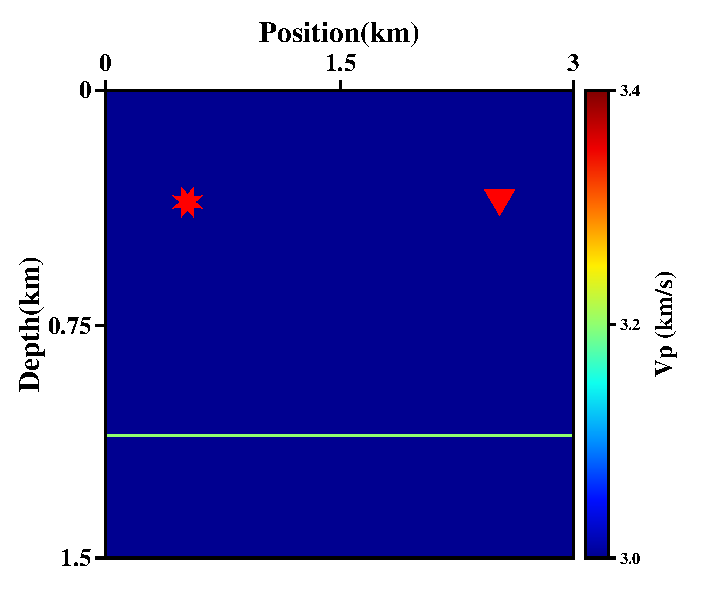
\includegraphics[width=0.5\textwidth]{Kernel/1vp.pdf}}
   \subfloat[]{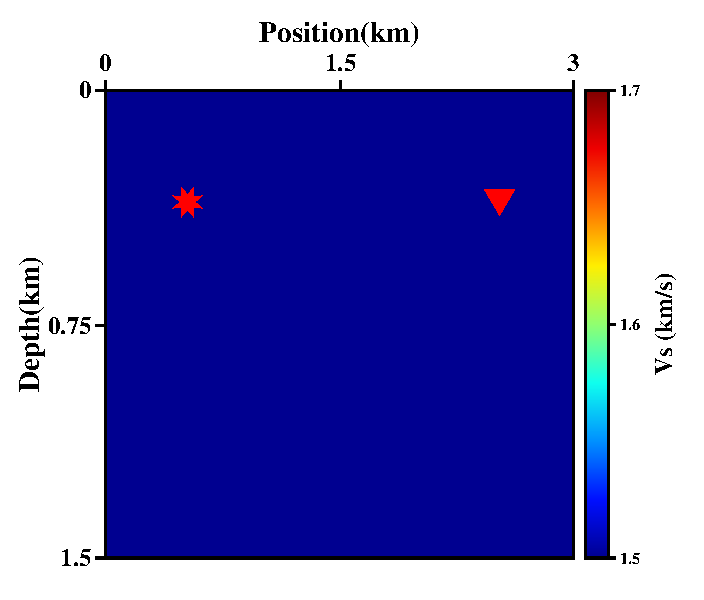
\includegraphics[width=0.5\textwidth]{Kernel/1vs.pdf}}\\
   \subfloat[]{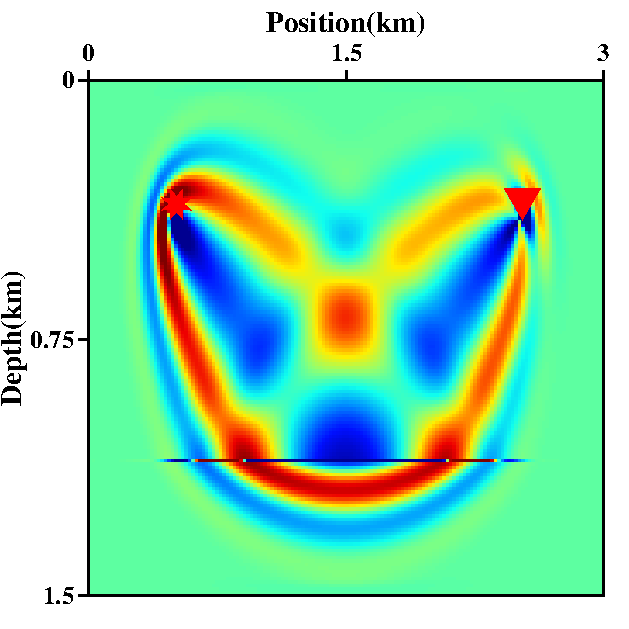
\includegraphics[width=0.5\textwidth]{Kernel/Vponlyvp.pdf}}
   \subfloat[]{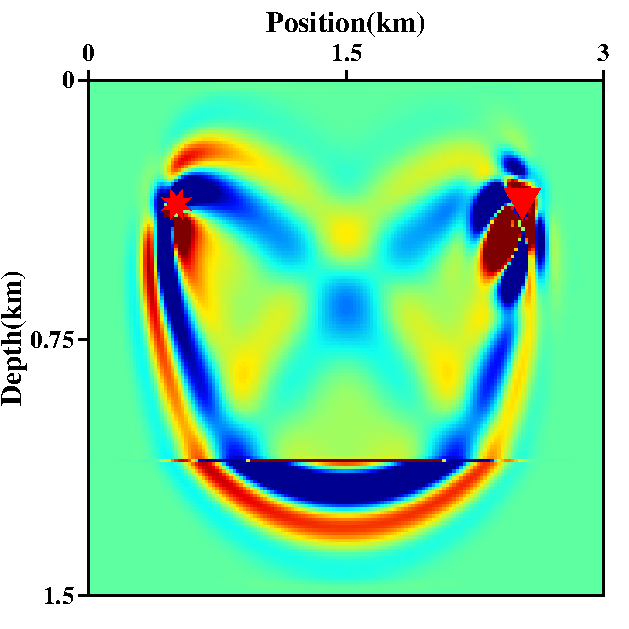
\includegraphics[width=0.5\textwidth]{Kernel/Vsonlyvp.pdf}}\\
   \caption{Kernels with single reflector in $V_p$ model. (a) $V_p$ model, (b) $V_s$ model, (c) $K_{V_p}$, (d) $K_{V_s}$.}
   \label{fig:kernel1_vp}
\end{figure}

\begin{figure}[!htb]
   \centering
   \subfloat[]{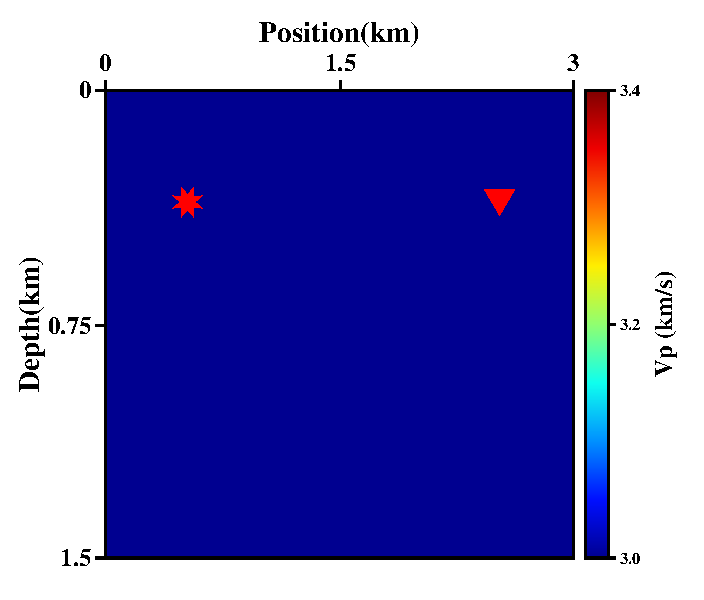
\includegraphics[width=0.50\textwidth]{Kernel/2vp.pdf}}
   \subfloat[]{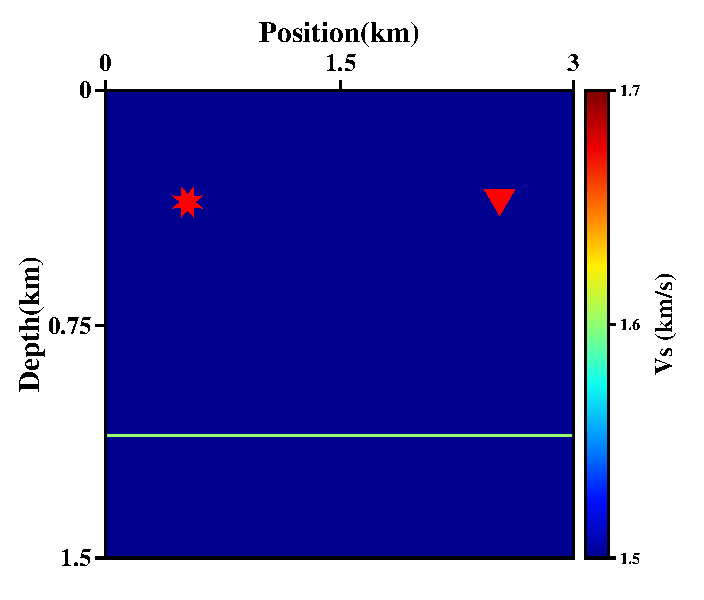
\includegraphics[width=0.50\textwidth]{Kernel/2vs.pdf}}\\
   \subfloat[]{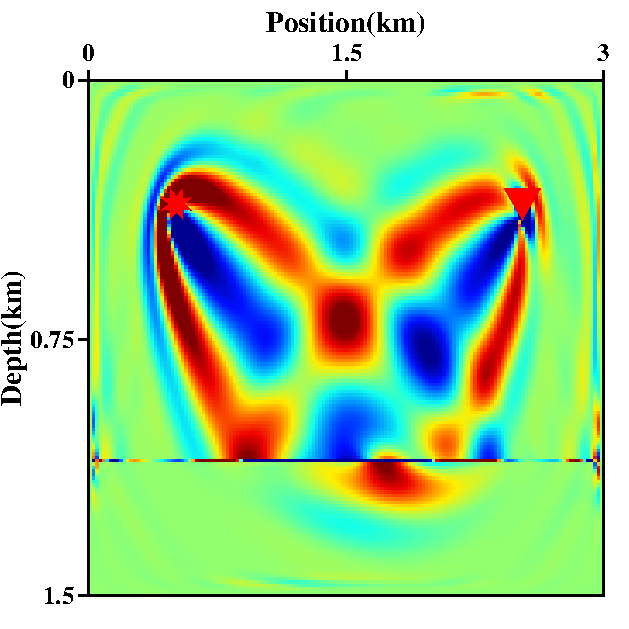
\includegraphics[width=0.50\textwidth]{Kernel/Vponlyvs.pdf}}
   \subfloat[]{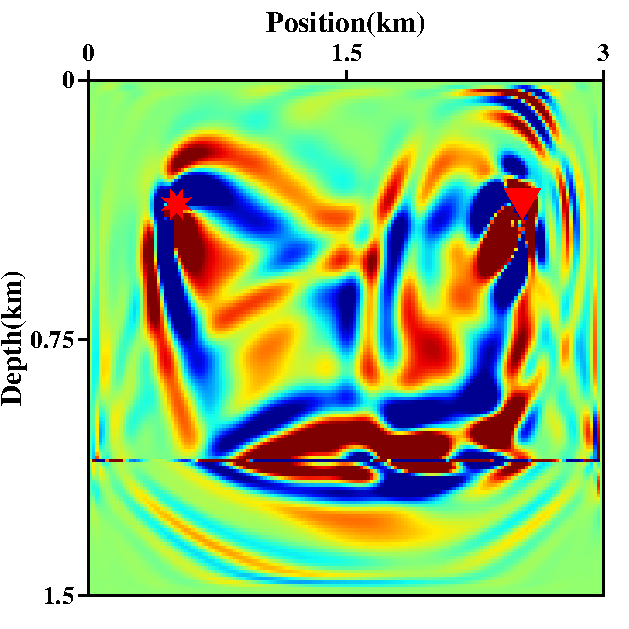
\includegraphics[width=0.50\textwidth]{Kernel/Vsonlyvs.pdf}}\\
   \caption{Kernels with single reflector in $V_s$ model. (a) $V_p$ model, (b) $V_s$ model, (c) $K_{V_p}$, (d) $K_{V_s}$.}
   \label{fig:kernel2}
\end{figure}

\begin{figure}[!htb]
   \centering
   \subfloat[]{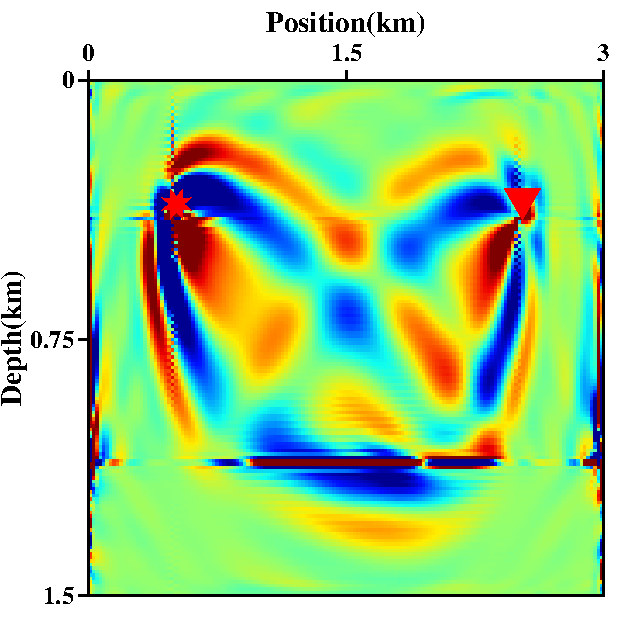
\includegraphics[width=0.50\textwidth]{Kernel/VsonlyvsPP.pdf}}
   \subfloat[]{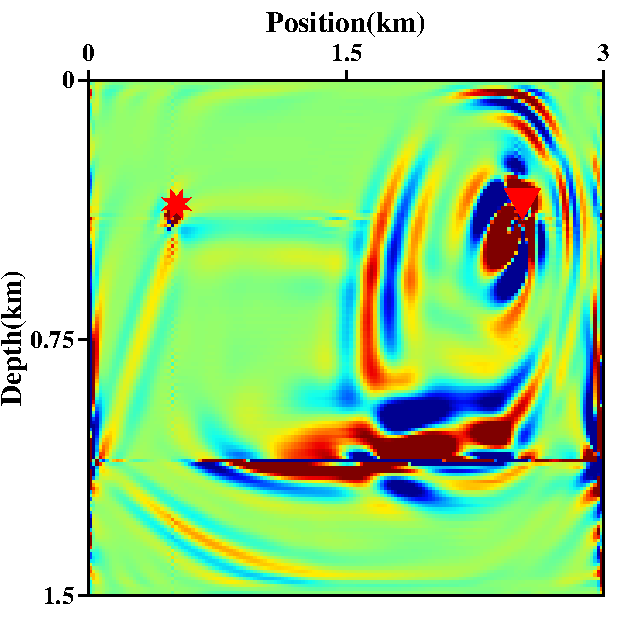
\includegraphics[width=0.50\textwidth]{Kernel/VsonlyvsPS.pdf}}\\
   \subfloat[]{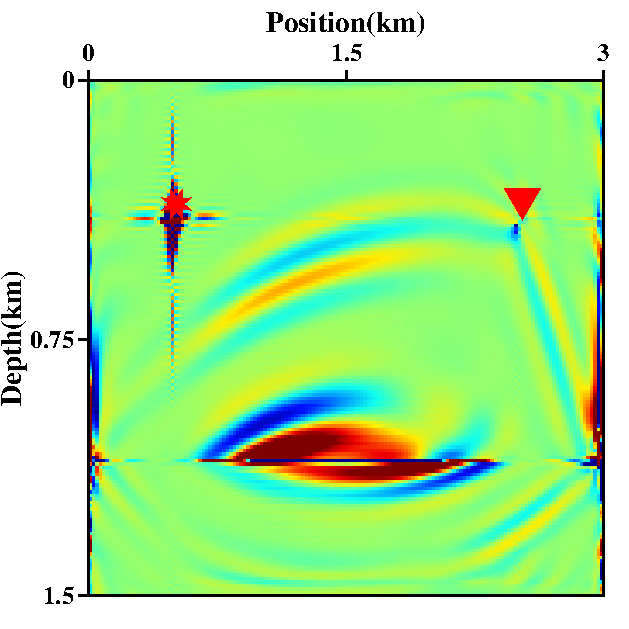
\includegraphics[width=0.50\textwidth]{Kernel/VsonlyvsSP.pdf}}
   \subfloat[]{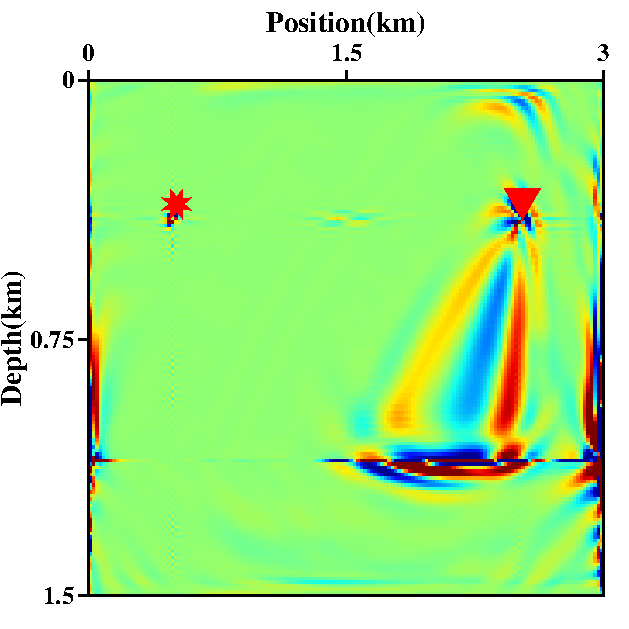
\includegraphics[width=0.50\textwidth]{Kernel/VsonlyvsSS.pdf}}
   \caption{Four components of $K_{V_s}$. (a) $K_{V_s}^{PP}$, (b) $K_{V_s}^{PS}$, (c) $K_{V_s}^{SP}$, (d) $K_{V_s}^{SS}$.}
   \label{fig:kernel2_vs_decomp}
\end{figure}

\begin{figure}
   \centering
   \subfloat{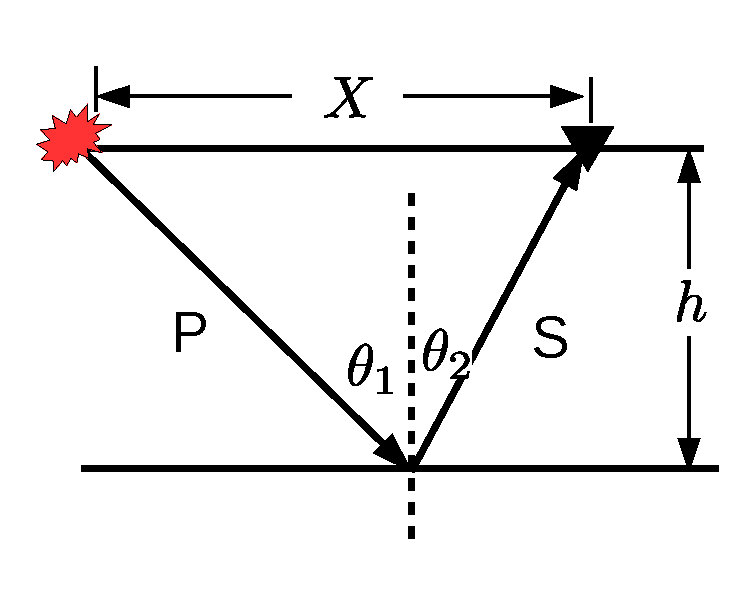
\includegraphics[width=0.40\textwidth]{PS_problem/PS_refl.pdf}}
   \caption{Ray path of PS reflection with a single reflector.}
   \label{fig:PS_refl}
\end{figure}

\begin{figure}
   \centering
   \subfloat[]{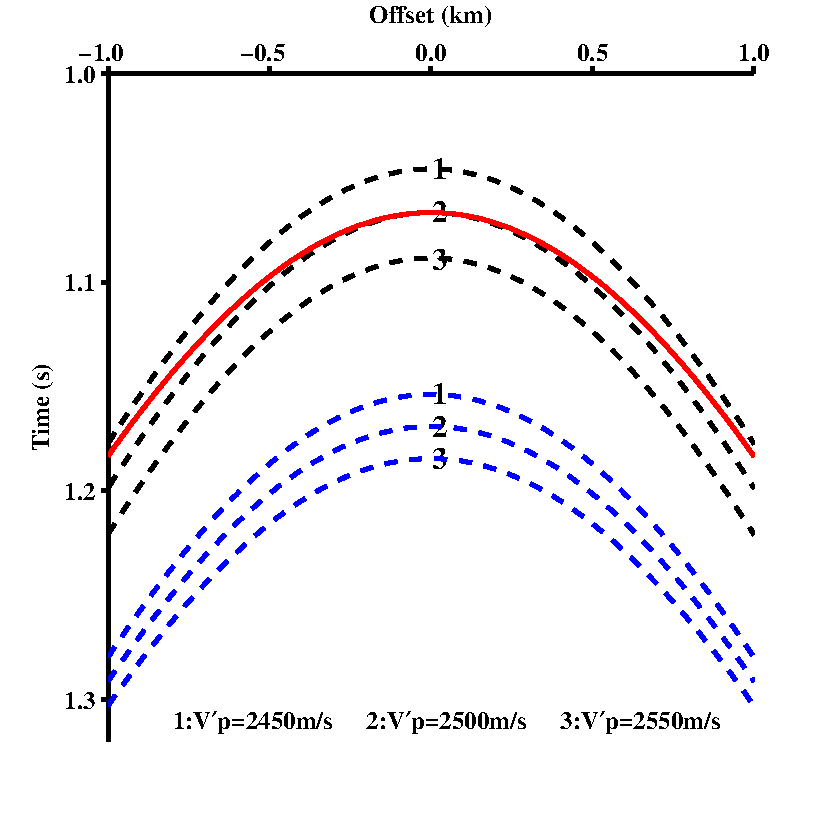
\includegraphics[width=0.5\textwidth]{PS_problem/h1000.pdf}}
   \subfloat[]{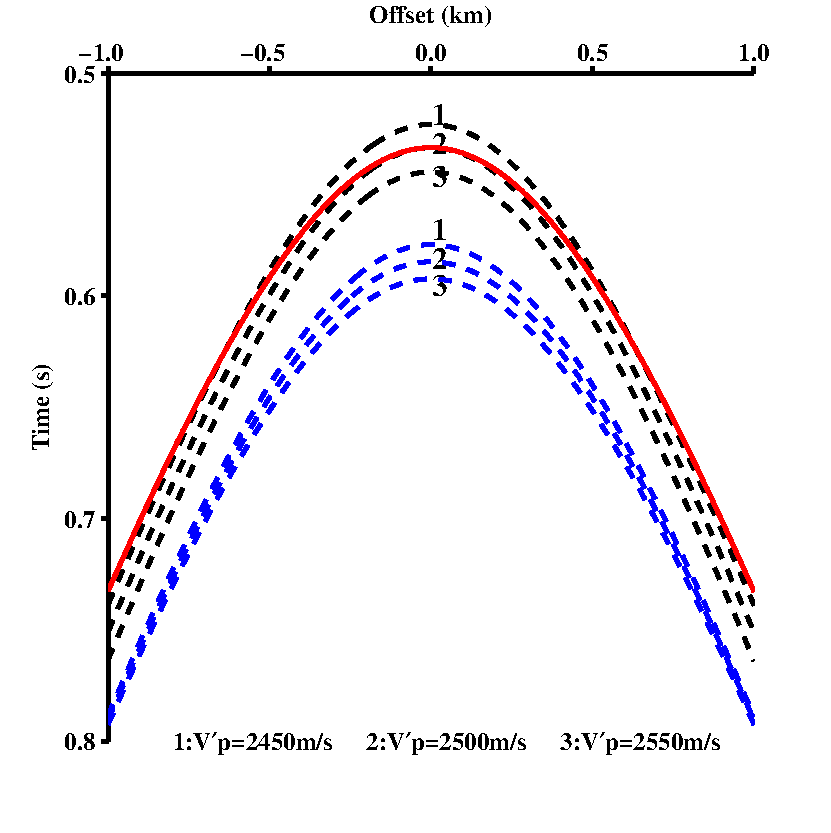
\includegraphics[width=0.5\textwidth]{PS_problem/h500.pdf}}
   \caption{The comparison among demigrated PS traveltime moveout of method \uppercase\expandafter{\romannumeral1} (black), method 
   \uppercase\expandafter{\romannumeral2} (blue) and the real (red) one.
   (a) $h=1000m$, (b) $h=500m$.}
   \label{fig:Sens_vp}
\end{figure}

\begin{figure}[!htb]
   \centering
   \subfloat{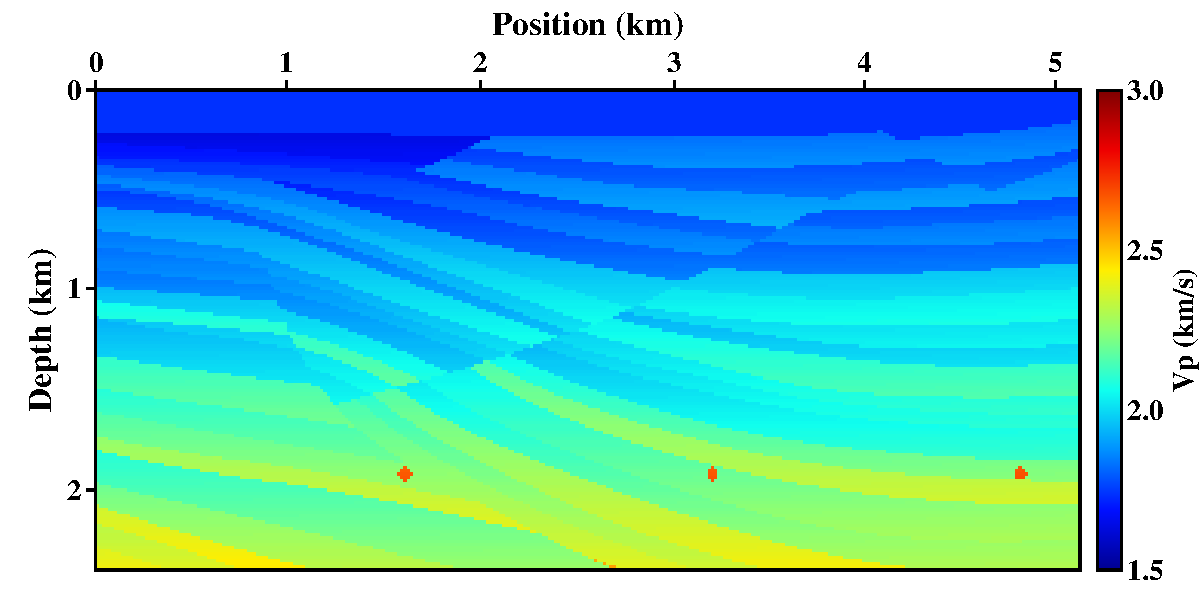
\includegraphics[width=0.5\textwidth]{sigbee2/Fig/cuttruevp.pdf}}
   \subfloat{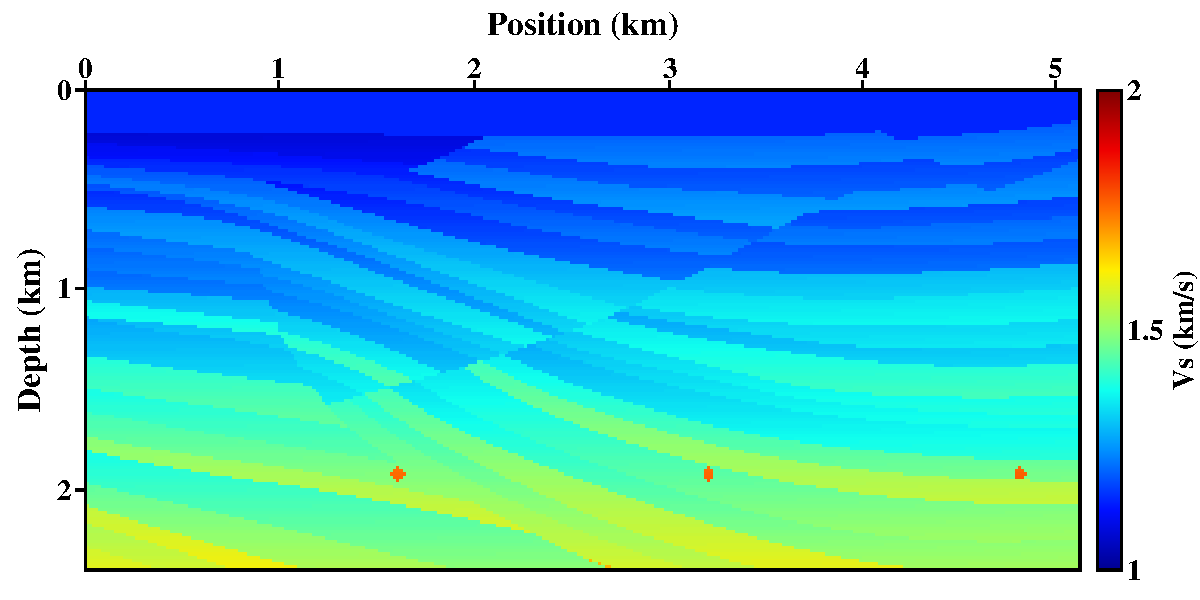
\includegraphics[width=0.5\textwidth]{sigbee2/Fig/cuttruevs.pdf}}\\
   \subfloat{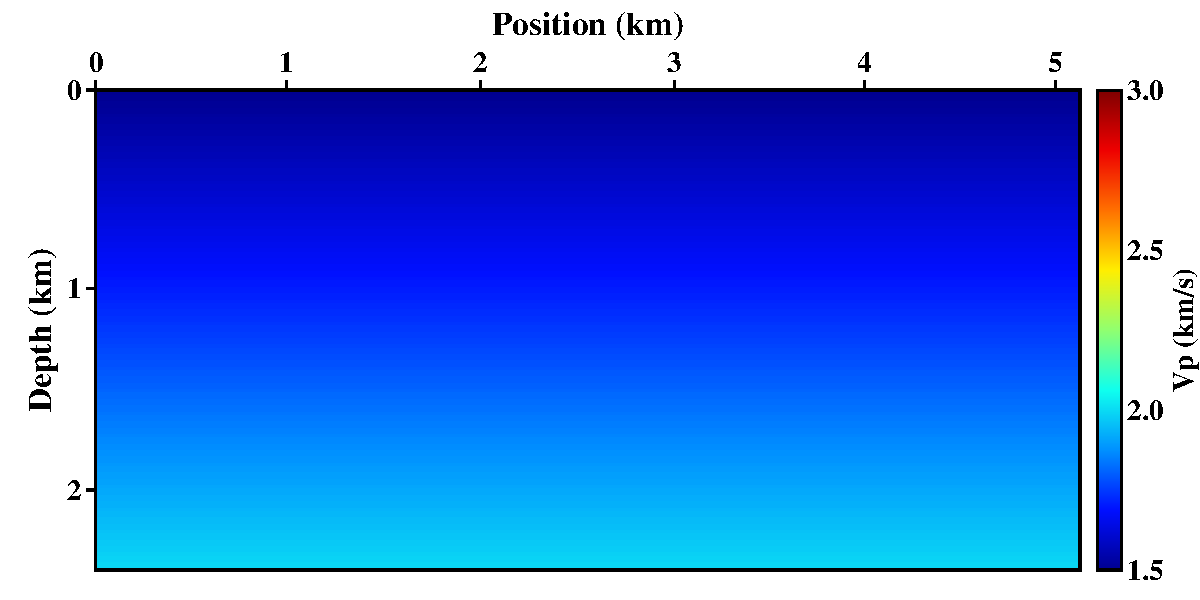
\includegraphics[width=0.5\textwidth]{sigbee2/Fig/cutinitvp.pdf}}
   \subfloat{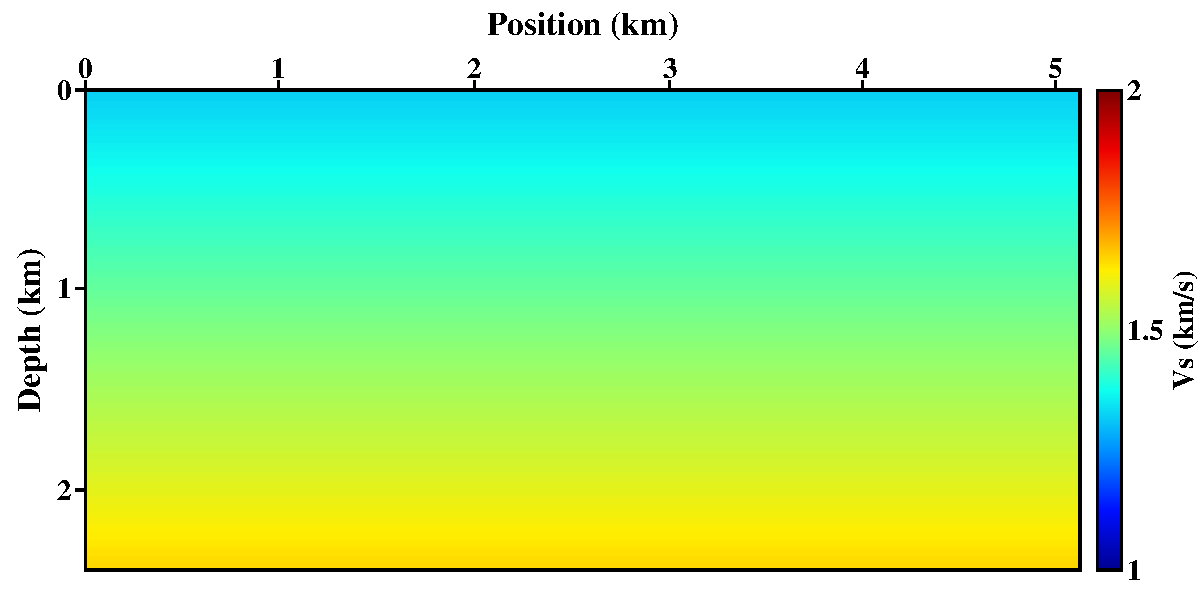
\includegraphics[width=0.5\textwidth]{sigbee2/Fig/cutinitvs.pdf}}
   \caption{Sigbee2A model example. On the top are true models of 
   $V_p$ (a) and $V_s$ (b). On the bottom are initial models of $V_p$ (c) and $V_s$
   (d) linearly increasing with depth. }
   \label{fig:TrueAndInitial}
\end{figure}

\begin{figure}
   \centering
   \subfloat[]{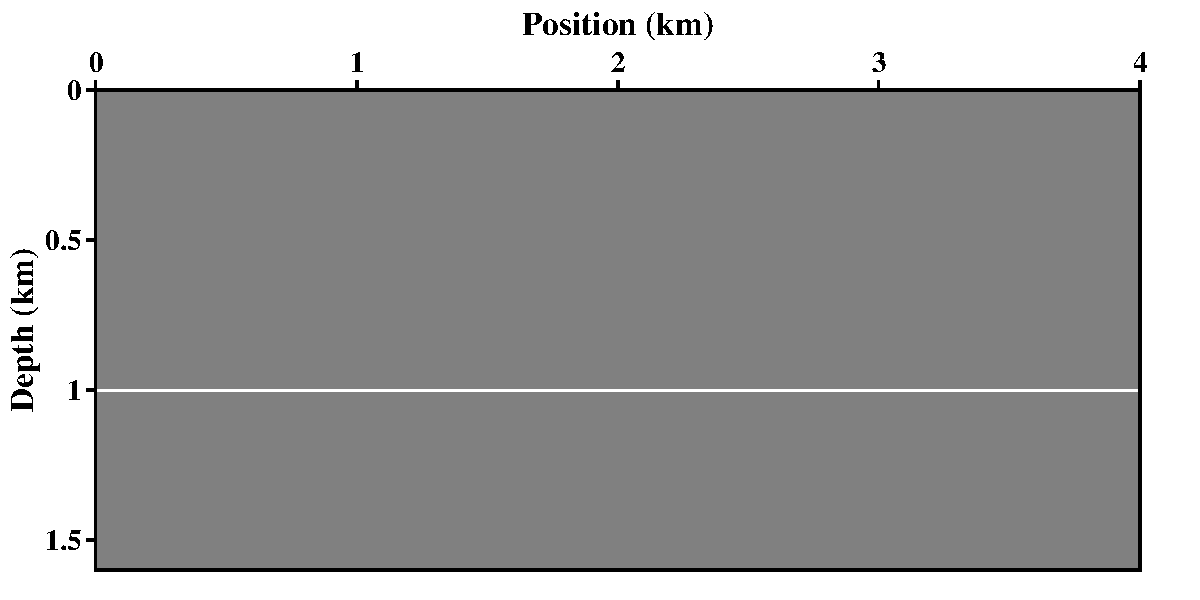
\includegraphics[width=0.5\textwidth]{DIW_L2/1layer.pdf}}
   \subfloat[]{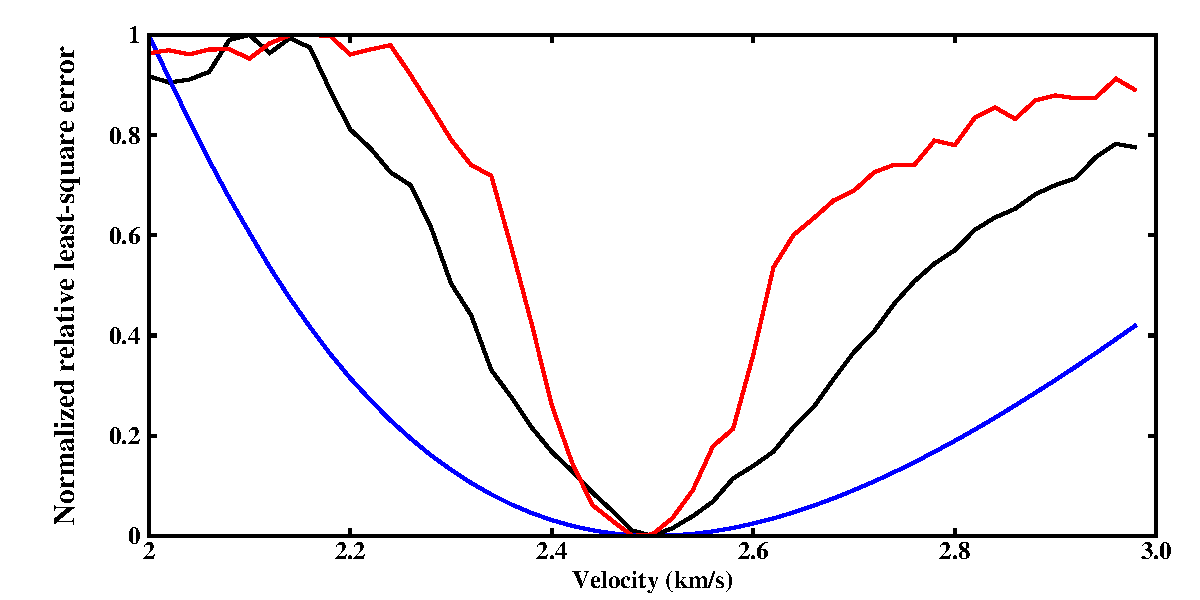
\includegraphics[width=0.5\textwidth]{DIW_L2/1layerL2.pdf}}\\
   \subfloat[]{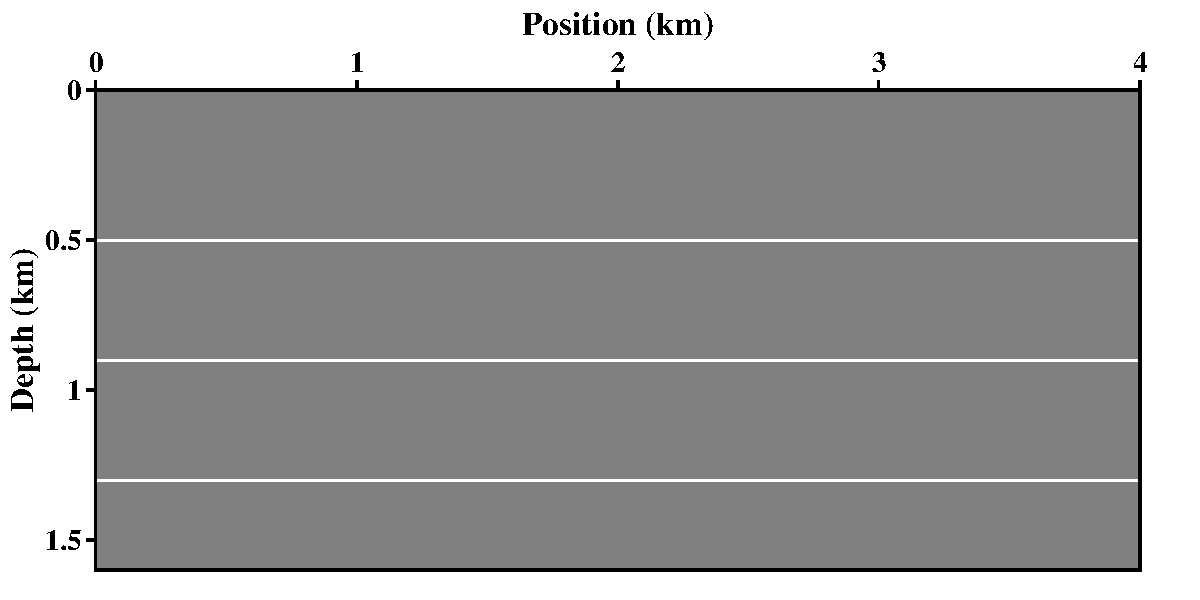
\includegraphics[width=0.5\textwidth]{DIW_L2/3layer.pdf}}
   \subfloat[]{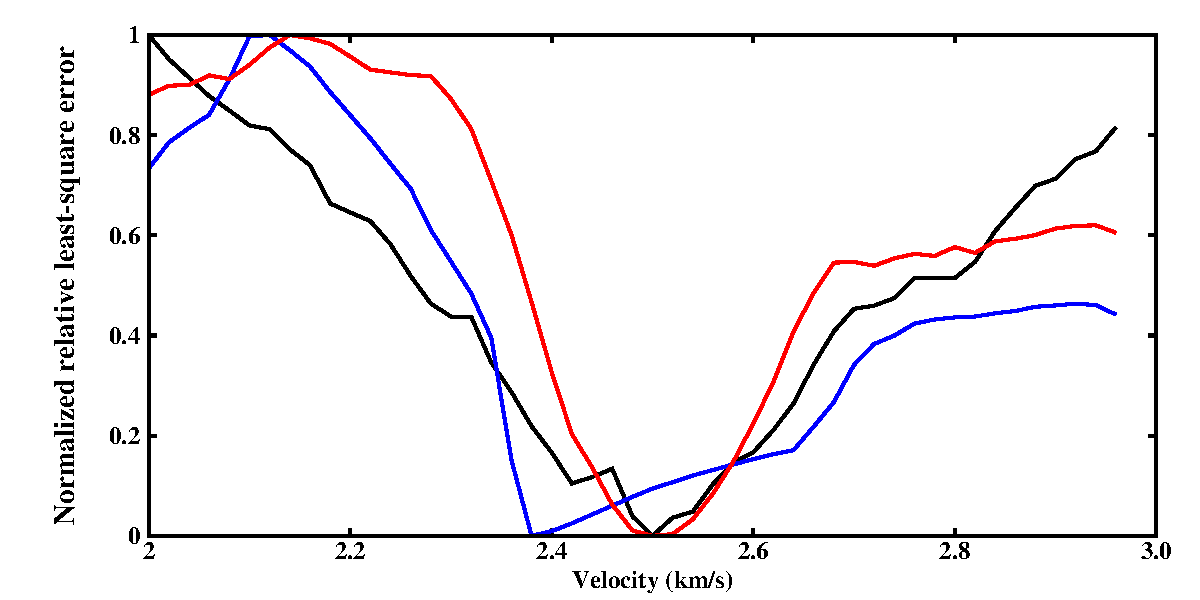
\includegraphics[width=0.5\textwidth]{DIW_L2/3layerL2.pdf}}\\
   \subfloat[]{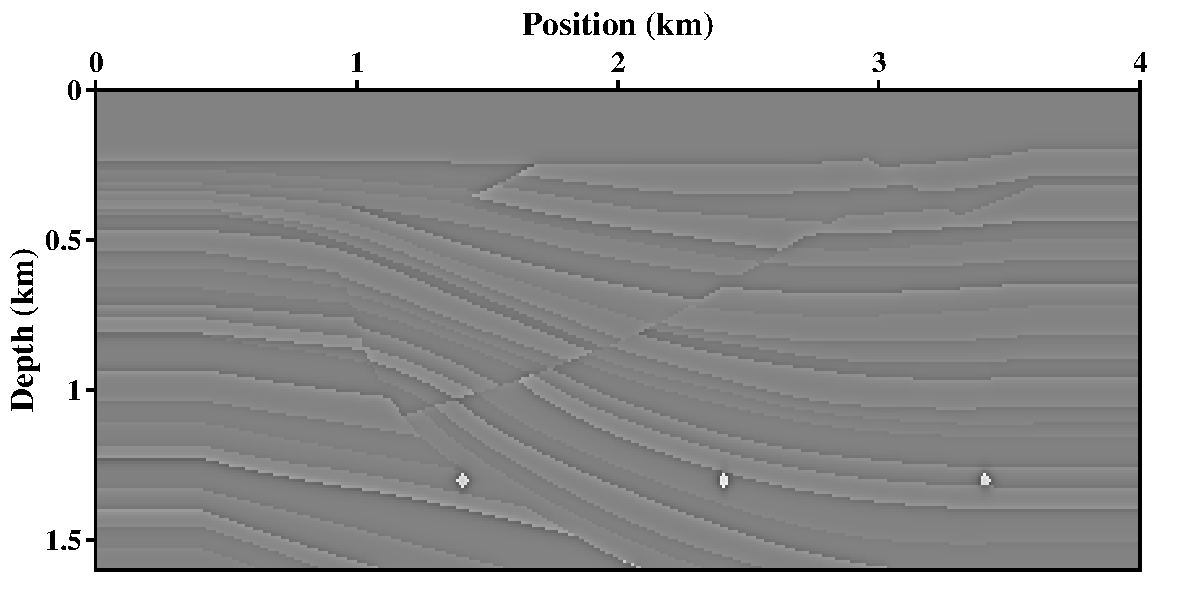
\includegraphics[width=0.5\textwidth]{DIW_L2/Sigsbee.pdf}}
   \subfloat[]{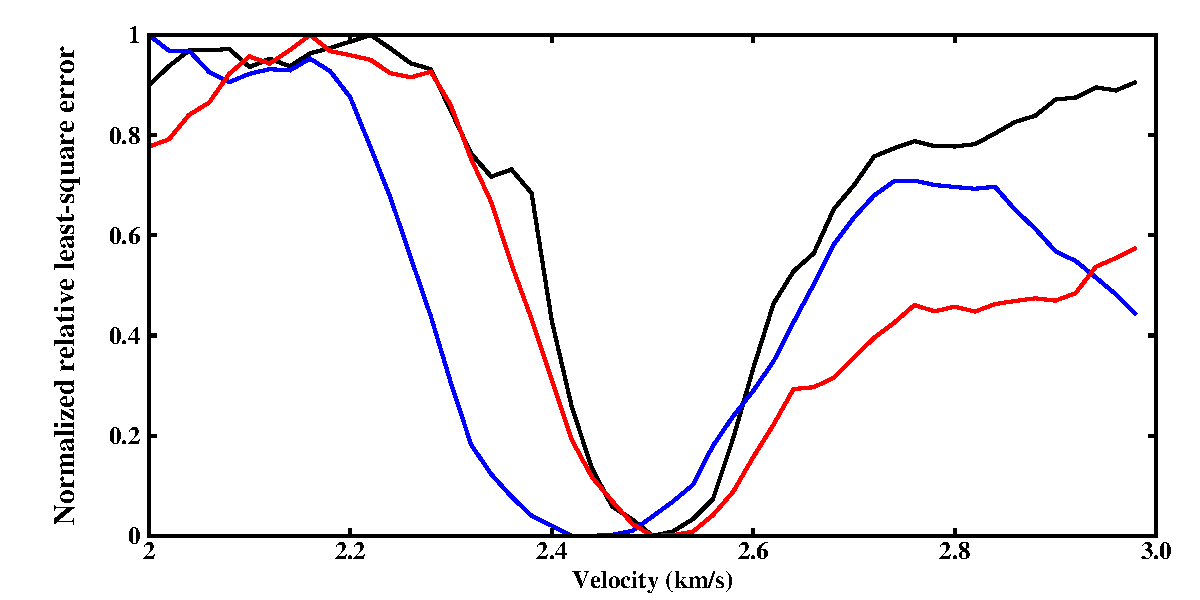
\includegraphics[width=0.5\textwidth]{DIW_L2/complexL2.pdf}}
   \caption{Normalized PP traveltime misfits for different objective functions for different model;}
   \label{fig:DIW_L2}
\end{figure}
\begin{figure}[!htb]
   \centering
   \subfloat[]{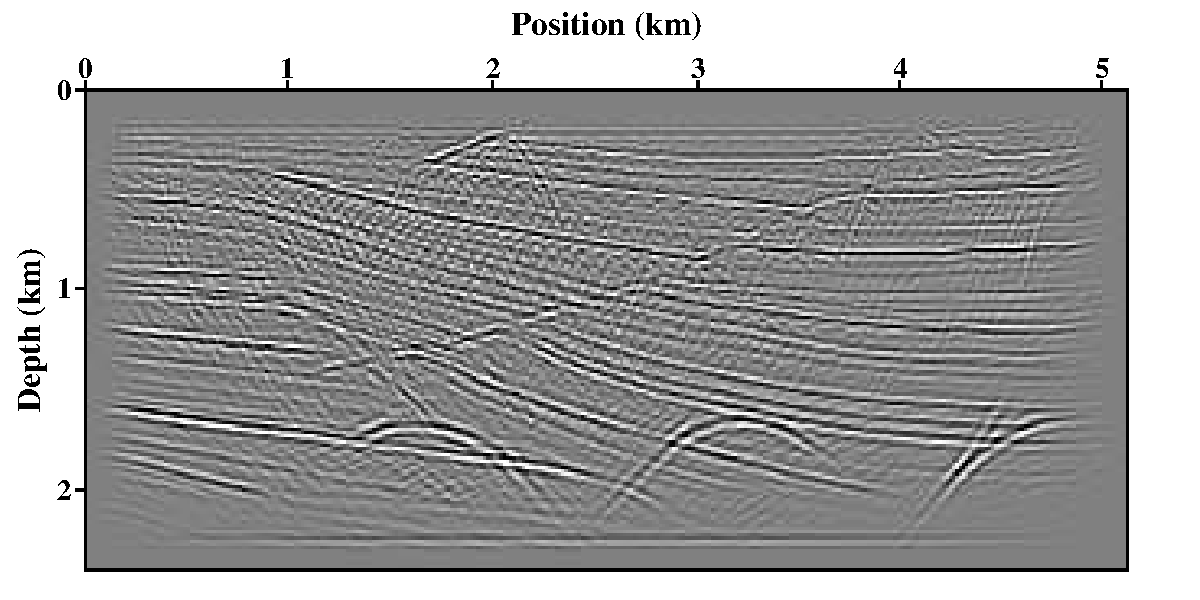
\includegraphics[width=0.5\textwidth]{sigbee2/Fig/cutimage_initvp.pdf}}
   \subfloat[]{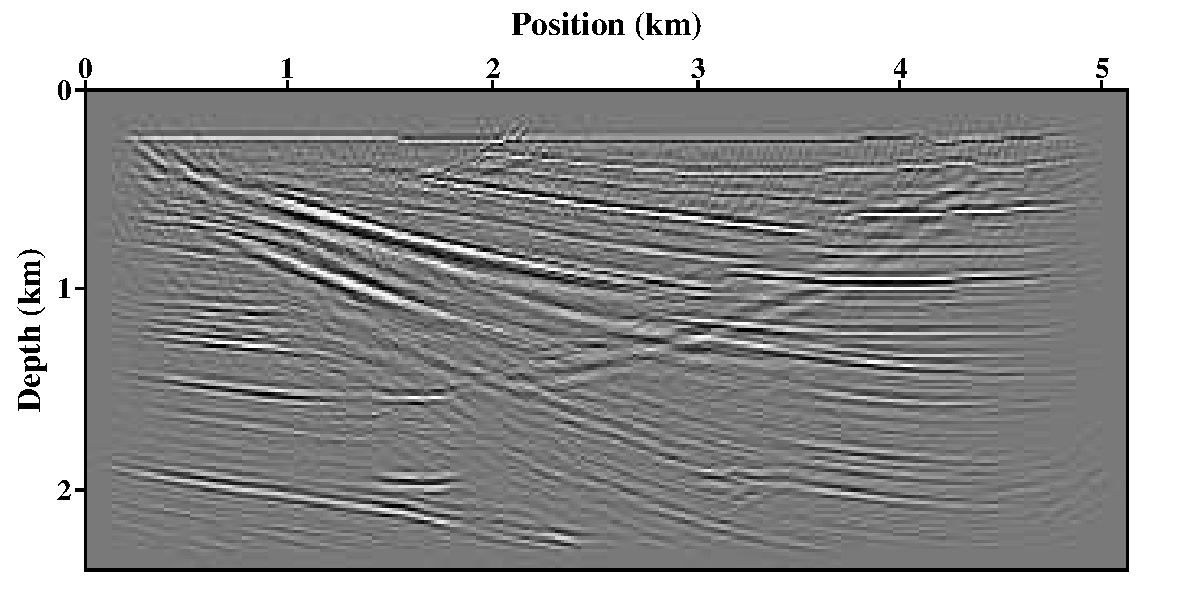
\includegraphics[width=0.5\textwidth]{sigbee2/Fig/cutimage_initvs.pdf}}\\
   \subfloat[]{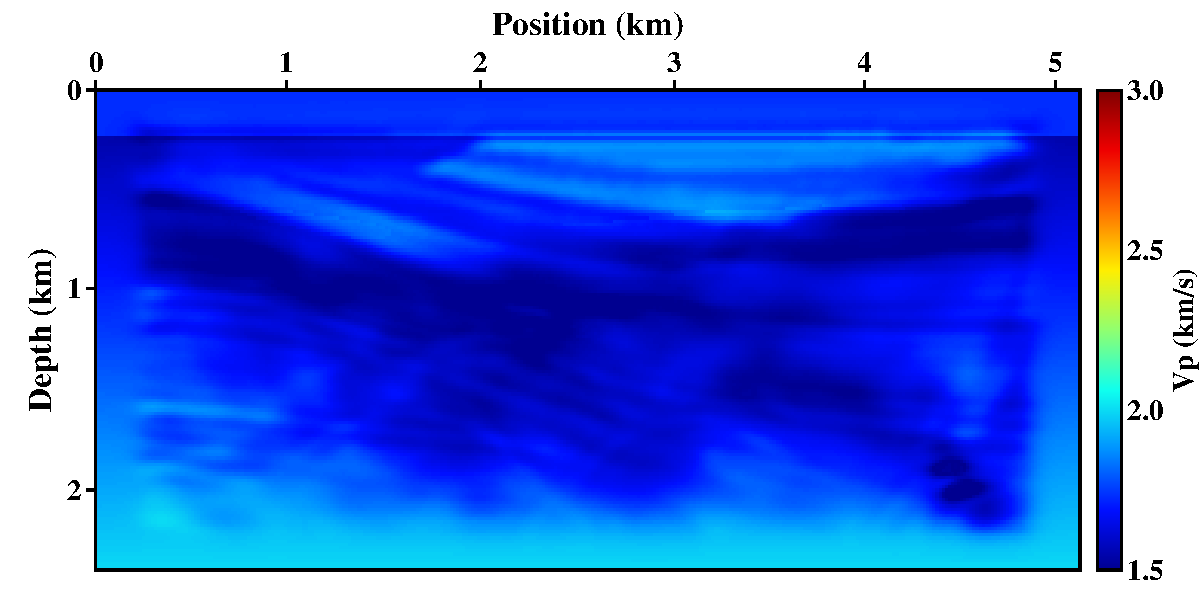
\includegraphics[width=0.5\textwidth]{sigbee2/badinitvp.pdf}}
   \subfloat[]{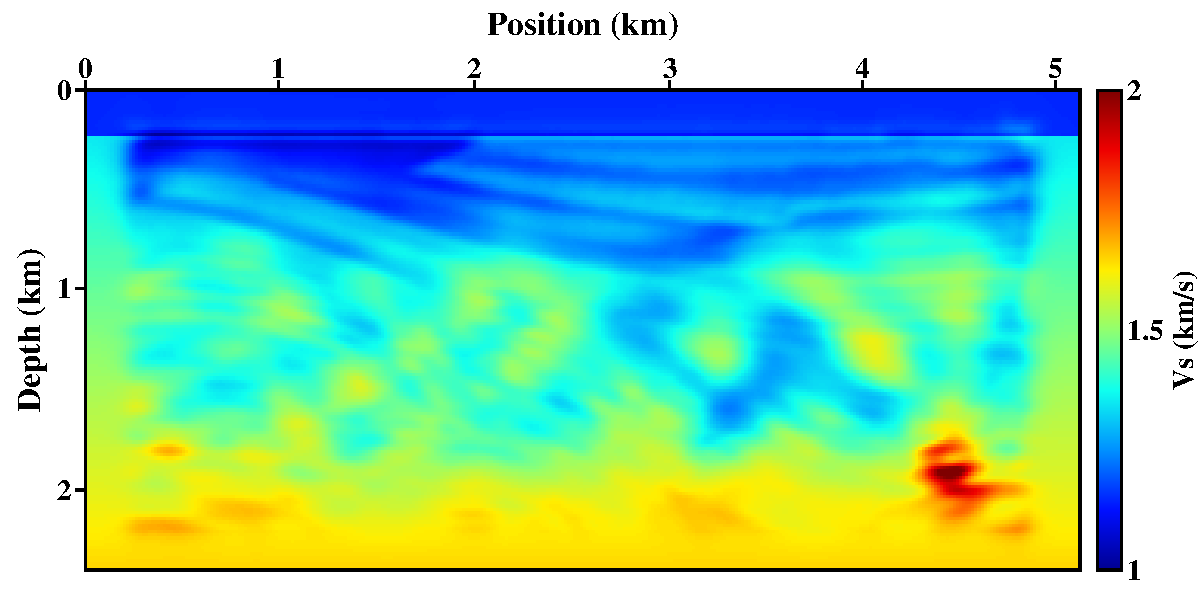
\includegraphics[width=0.5\textwidth]{sigbee2/badinitvs.pdf}}\\
   \caption{The results of ERTM and EFWI using initial model: (a) and (b) are PP and
   PS image of ERTM with near offset data, (c) and (d) are inverted $V_p$ and $V_s$
   with EFWI.}
   \label{fig:Results_init}
\end{figure}
\begin{figure}[!htb]
   \centering
   \subfloat[]{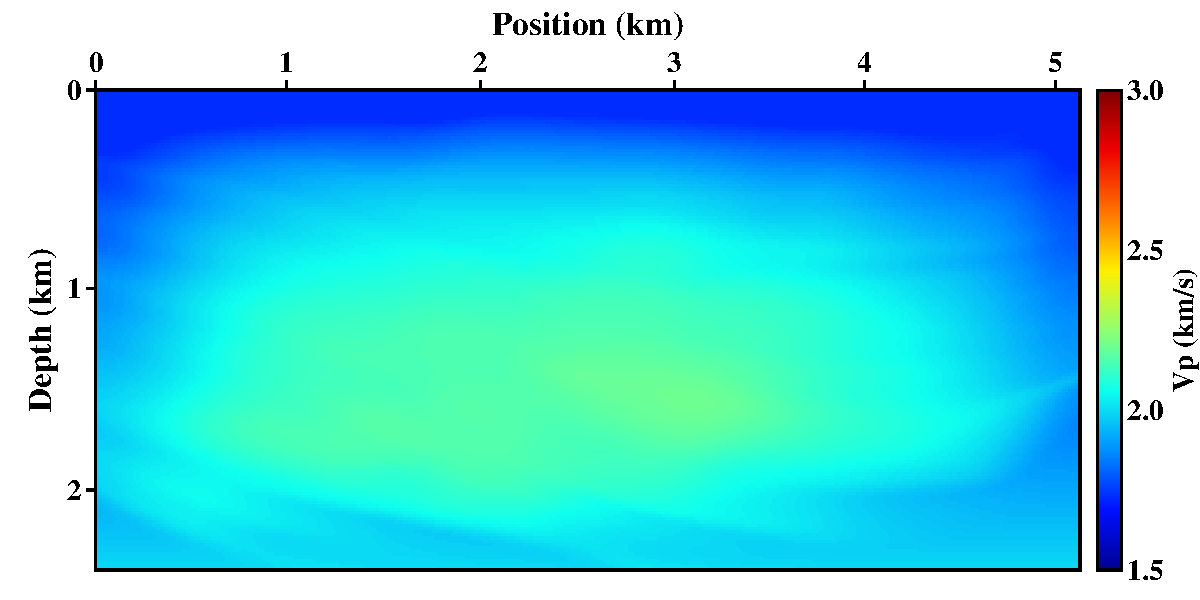
\includegraphics[width=0.5\textwidth]{sigbee2/Fig/newinit3vp.pdf}}
   \subfloat[]{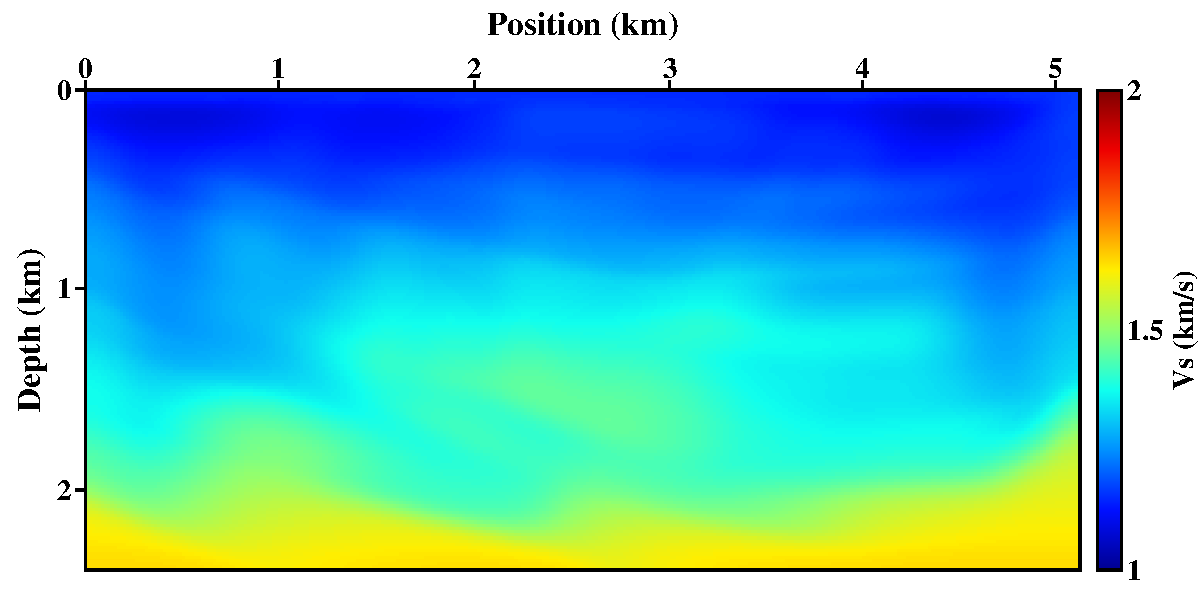
\includegraphics[width=0.5\textwidth]{sigbee2/Fig/newinit3vs.pdf}}\\
   \caption{Inverted results of ERTI: (a) $V_p$, (b) $V_s$.}
   \label{fig:InvertedModel_ERTI}
\end{figure}
\begin{figure}[!htb]
   \centering
   \subfloat[]{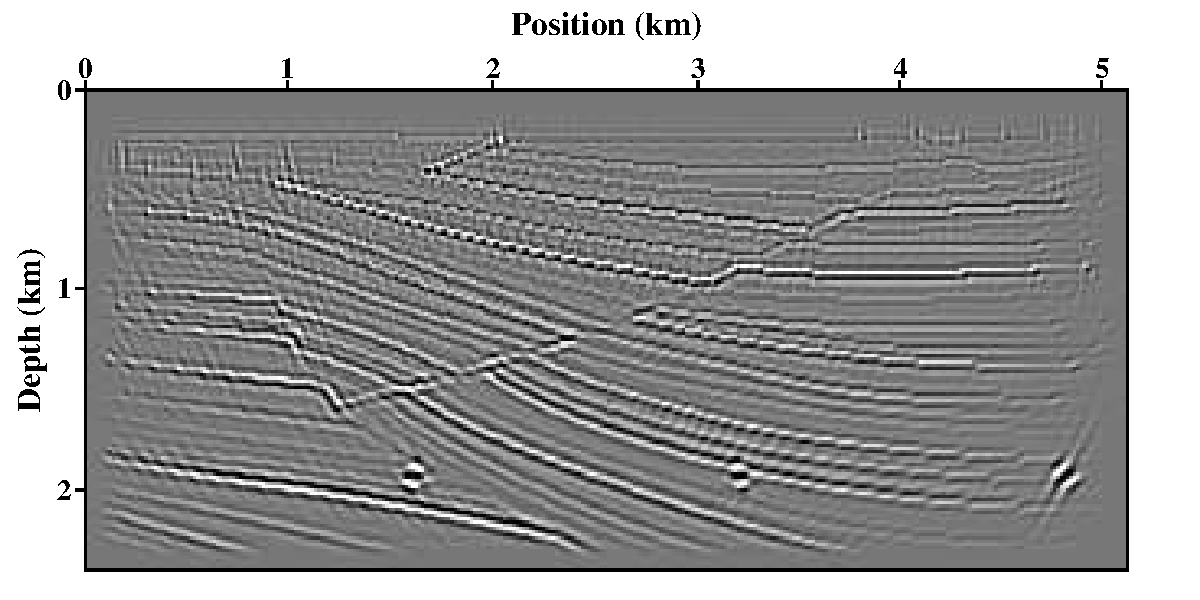
\includegraphics[width=0.5\textwidth]{sigbee2/Fig/cutimage_truevp.pdf}}
   \subfloat[]{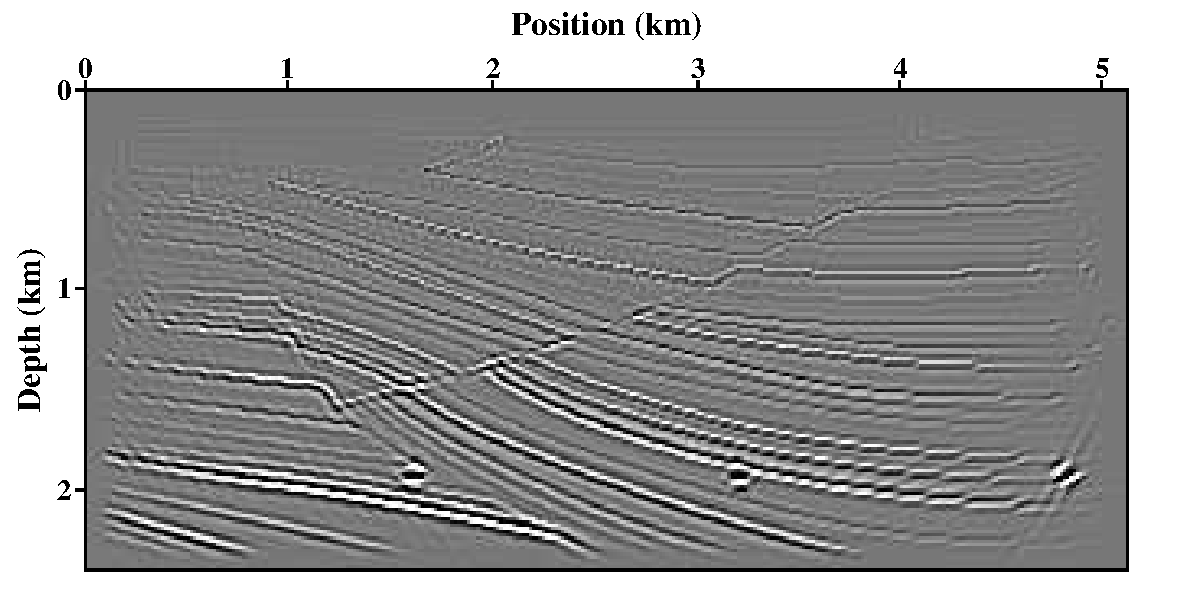
\includegraphics[width=0.5\textwidth]{sigbee2/Fig/cutimage_truevs.pdf}}\\
   \subfloat[]{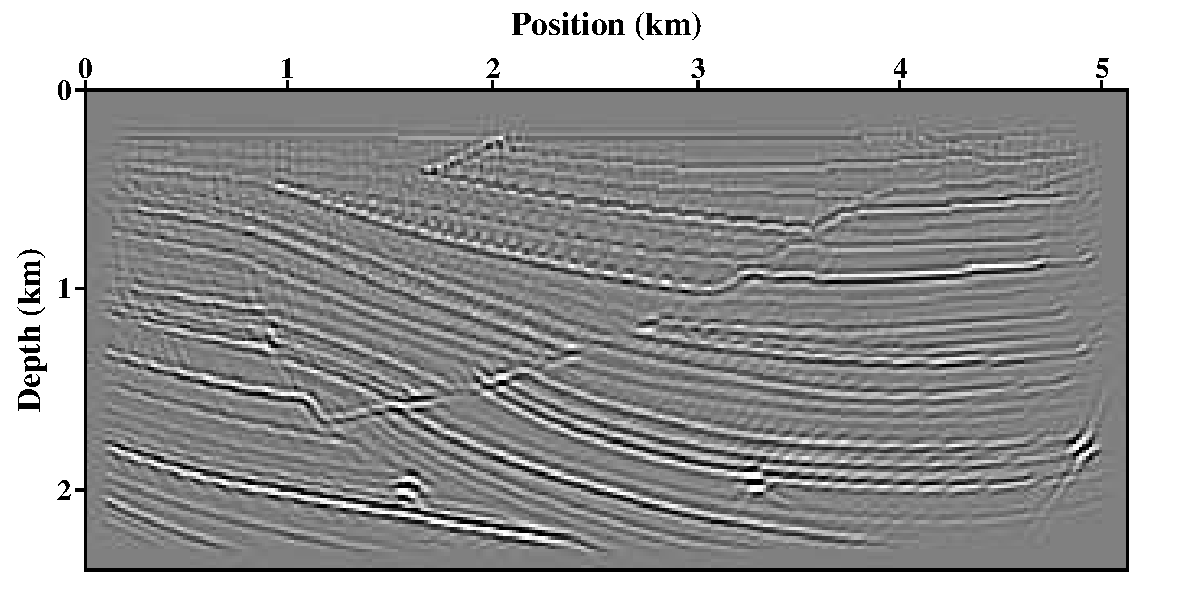
\includegraphics[width=0.5\textwidth]{sigbee2/Fig/cutimage_wertivp.pdf}}
   \subfloat[]{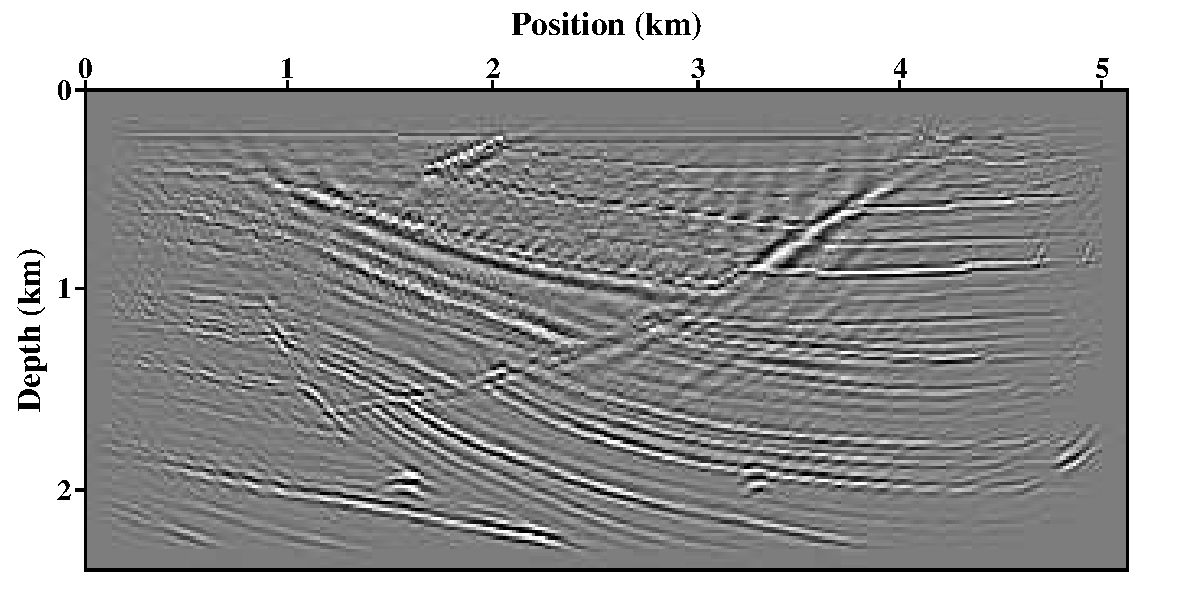
\includegraphics[width=0.5\textwidth]{sigbee2/Fig/cutimage_wertivs.pdf}}
   \caption{ERTM results using the true model (a, b) and
   inverted model (c, d). (a) and (c) are the PP image;(b) and (d) are the PS
   image}
   \label{fig:ERTM_comparison}
\end{figure}
\begin{figure}[!htb]
   \centering
   \subfloat[]{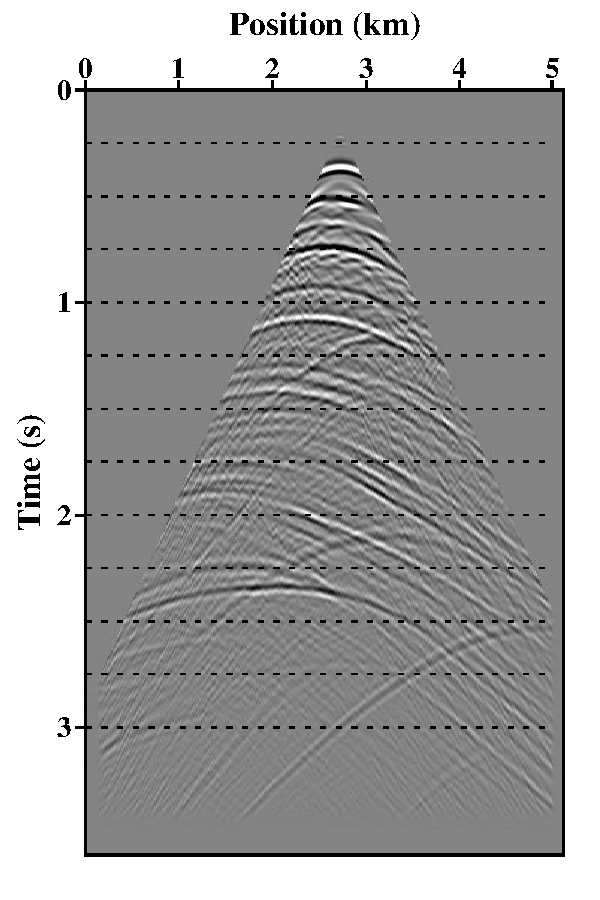
\includegraphics[width=0.33\textwidth]{sigbee2/Fig/DataPP_true.pdf}}
   \subfloat[]{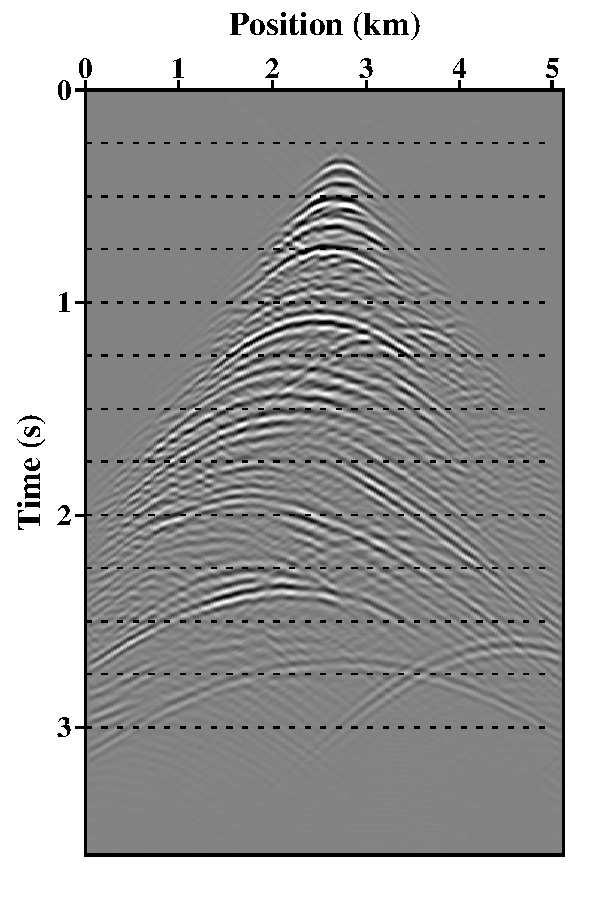
\includegraphics[width=0.33\textwidth]{sigbee2/Fig/DataPP_init.pdf}}
   \subfloat[]{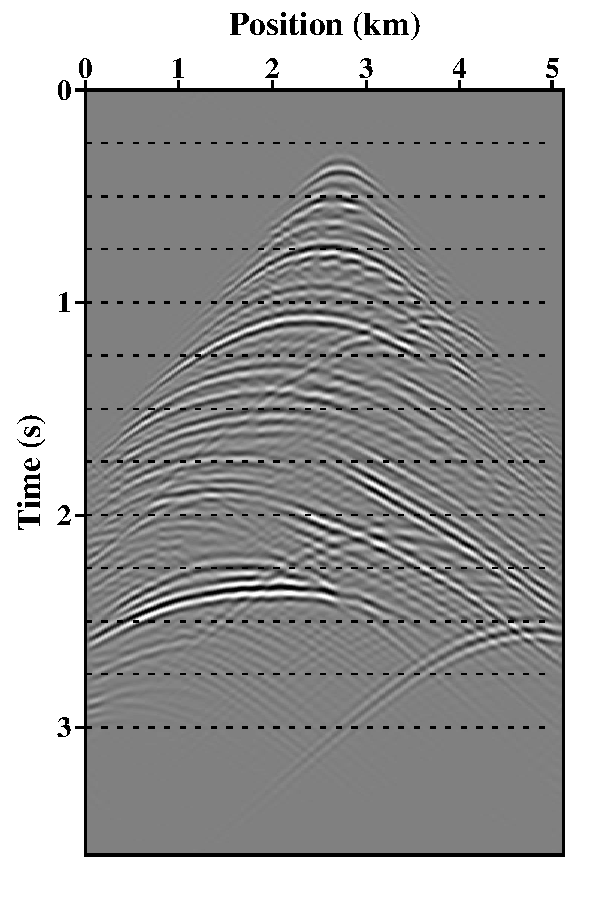
\includegraphics[width=0.33\textwidth]{sigbee2/Fig/DataPP_werti.pdf}}\\
   \subfloat[]{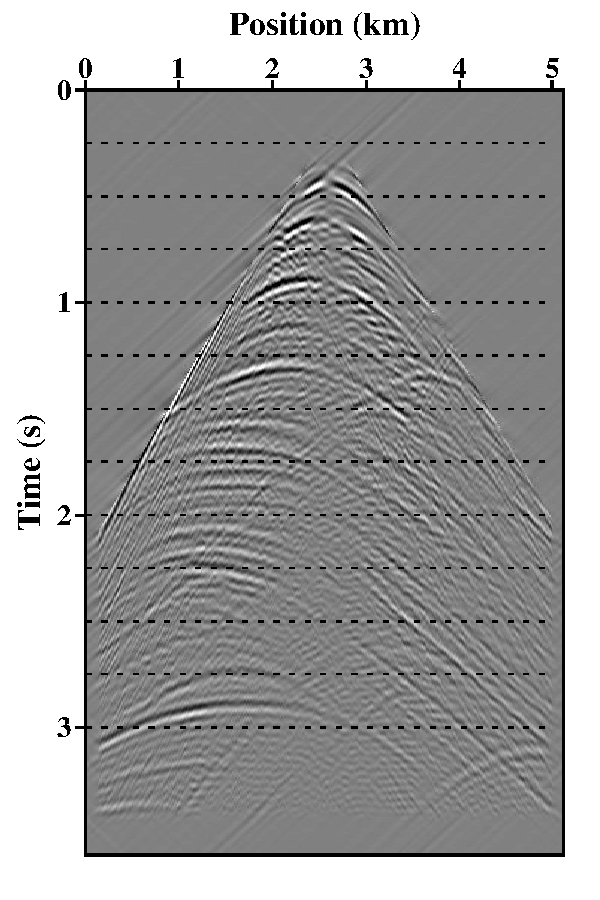
\includegraphics[width=0.33\textwidth]{sigbee2/Fig/DataPS_true.pdf}}
   \subfloat[]{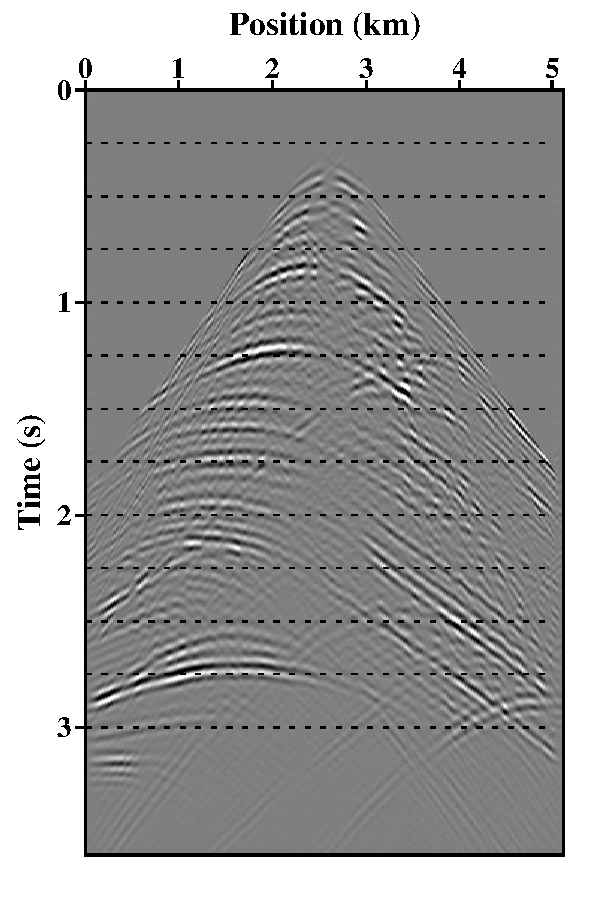
\includegraphics[width=0.33\textwidth]{sigbee2/Fig/DataPS_init.pdf}}
   \subfloat[]{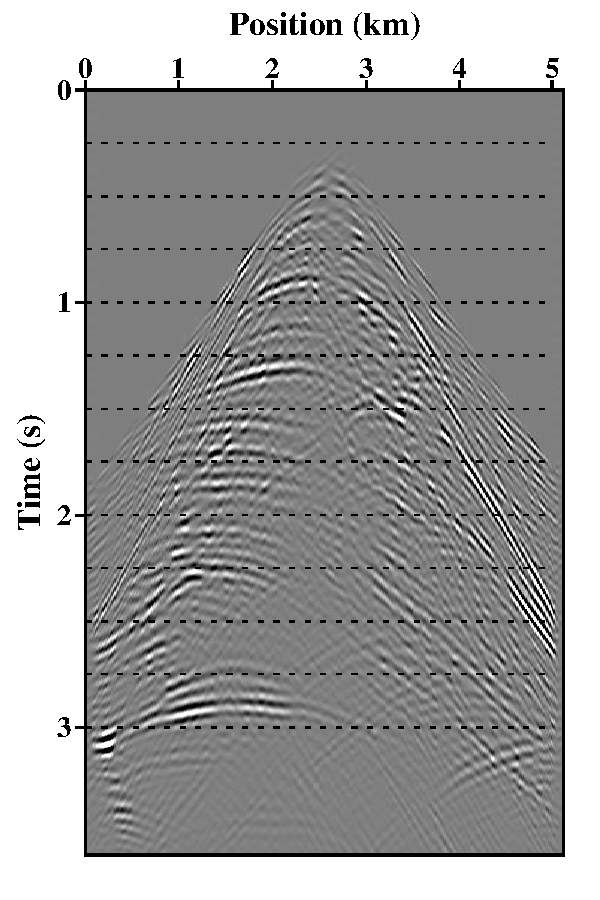
\includegraphics[width=0.33\textwidth]{sigbee2/Fig/DataPS_werti.pdf}}
   \caption{Comparison of the observed and the demigrated reflection data using
   initial model and the inverted model. The first row are the separated PP
   reflection, while the second row are the separated PS reflection. 
   The left, middle and right column are the observed reflection data, the
   demigrated reflection data with initial model
   and the demigrated data with inverted model, respectively. }
   \label{fig:Data_comparison}
\end{figure}
\begin{figure}[!htb]
   \centering
   \subfloat[]{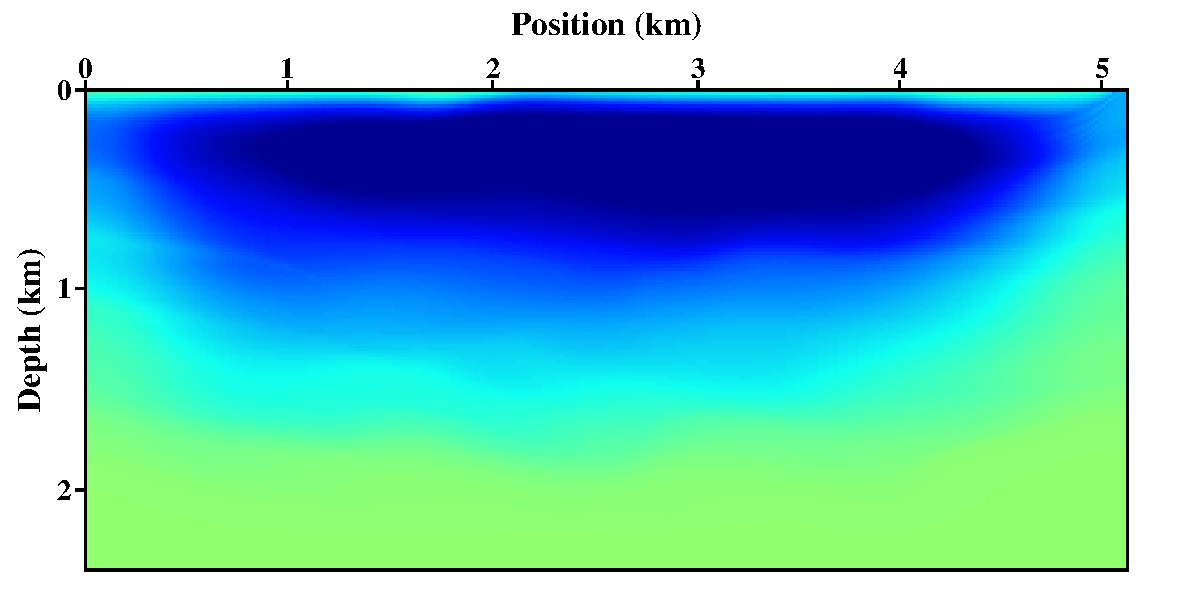
\includegraphics[width=0.5\textwidth]{sigbee2/LSF_Gra_vp.pdf}}
   \subfloat[]{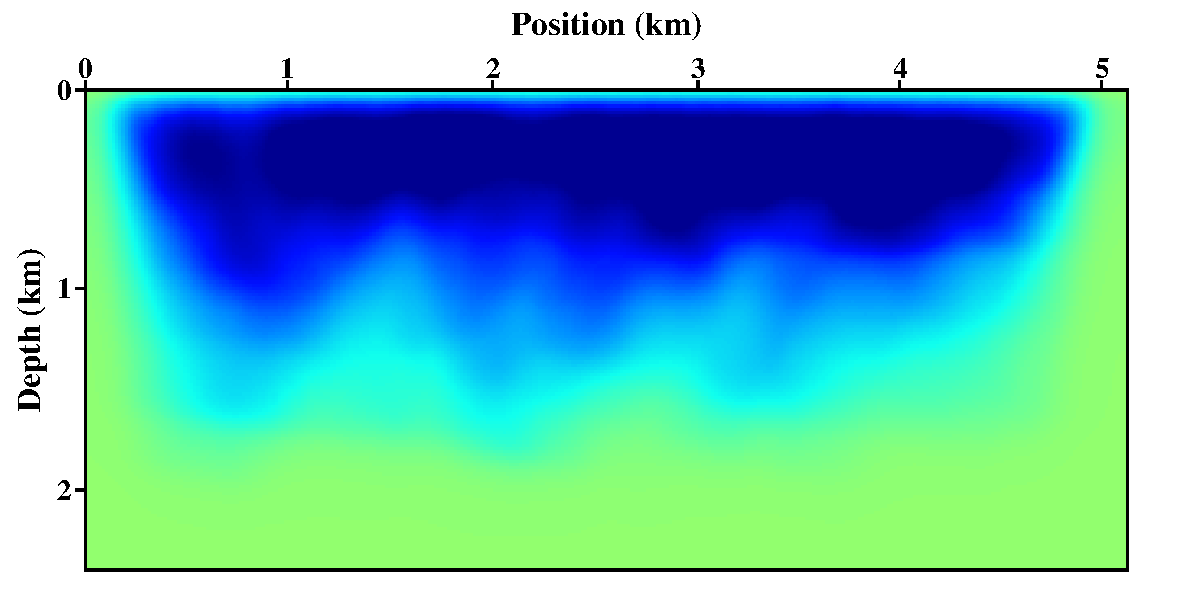
\includegraphics[width=0.5\textwidth]{sigbee2/NoLSF_Gra_vp.pdf}}\\
   \subfloat[]{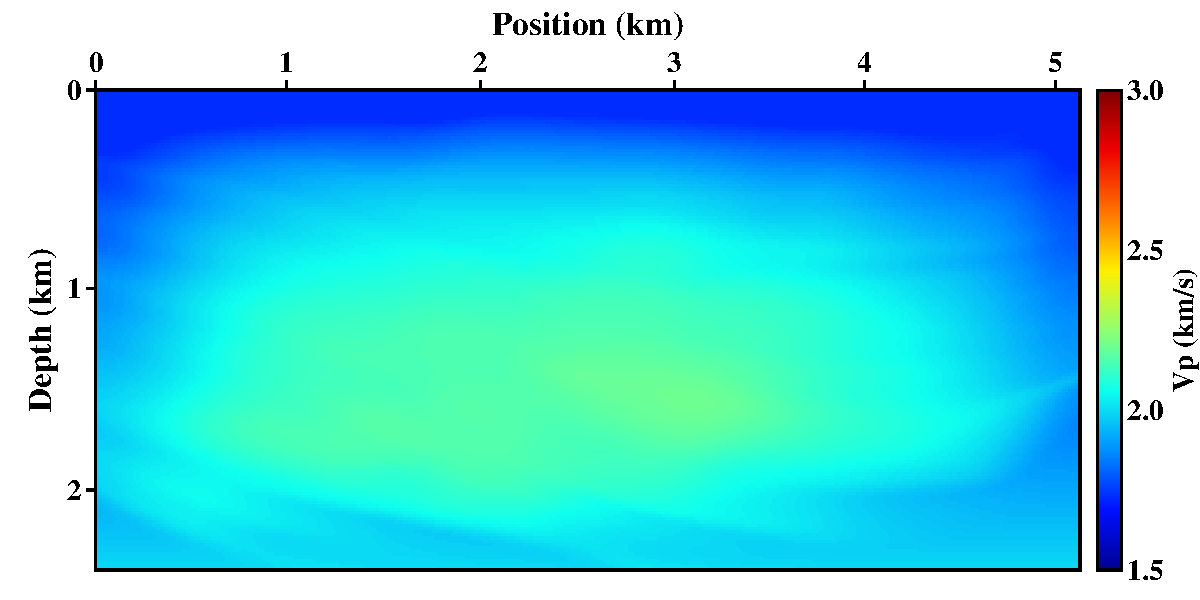
\includegraphics[width=0.5\textwidth]{sigbee2/Fig/newinit3vp.pdf}}
   \subfloat[]{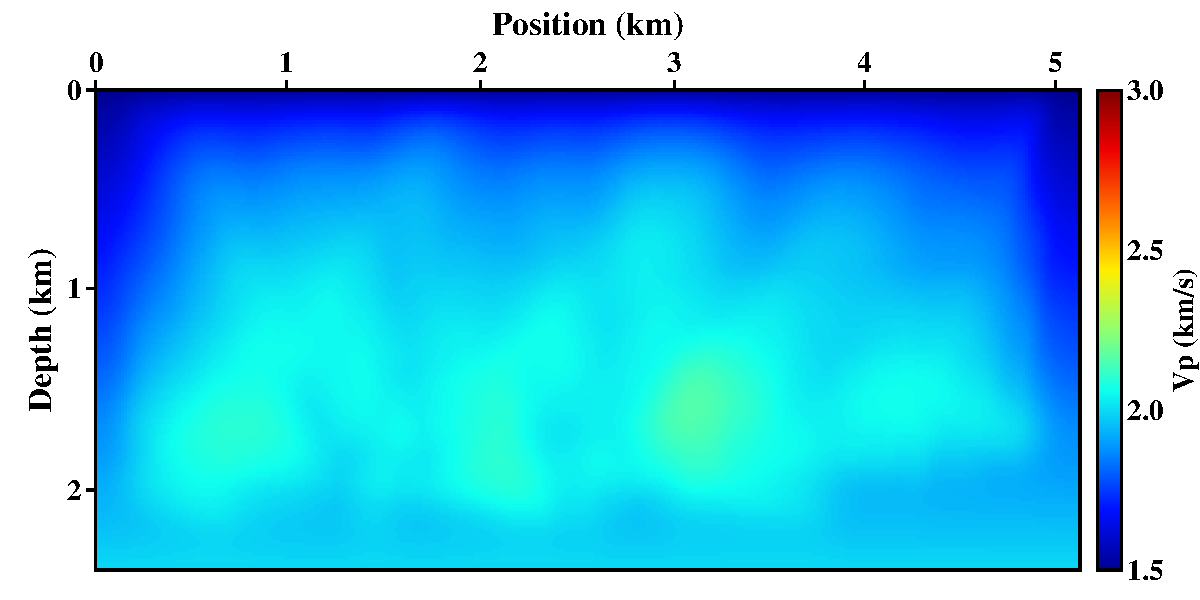
\includegraphics[width=0.5\textwidth]{sigbee2/NoLSF_vp.pdf}}\\
   \caption{The comparison of gradients and final inverted results with (left) and
   without (right) 
   the structure-oriented constrain: (a) and (c) are the $V_p$ gradients in the first
   iteration, (b) and (d) are final inverted $V_p$ model.}
   \label{fig:LSF_comparison}
\end{figure}

\begin{figure}[!htb]
   \centering
   \subfloat[]{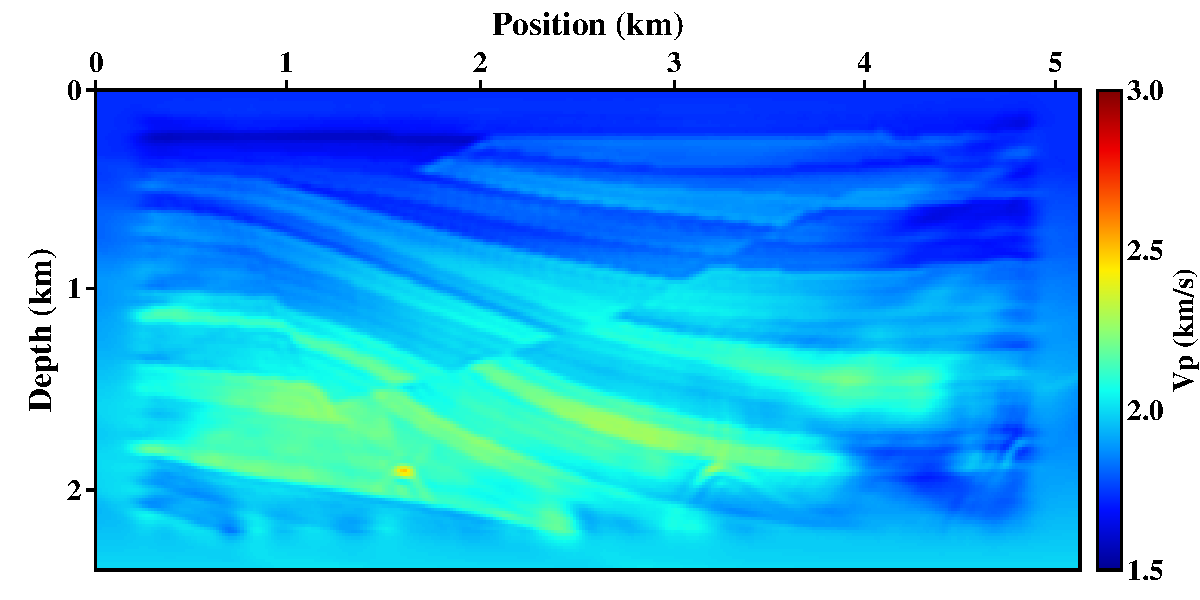
\includegraphics[width=0.5\textwidth]{sigbee2/Fig/nodevp.pdf}}
   \subfloat[]{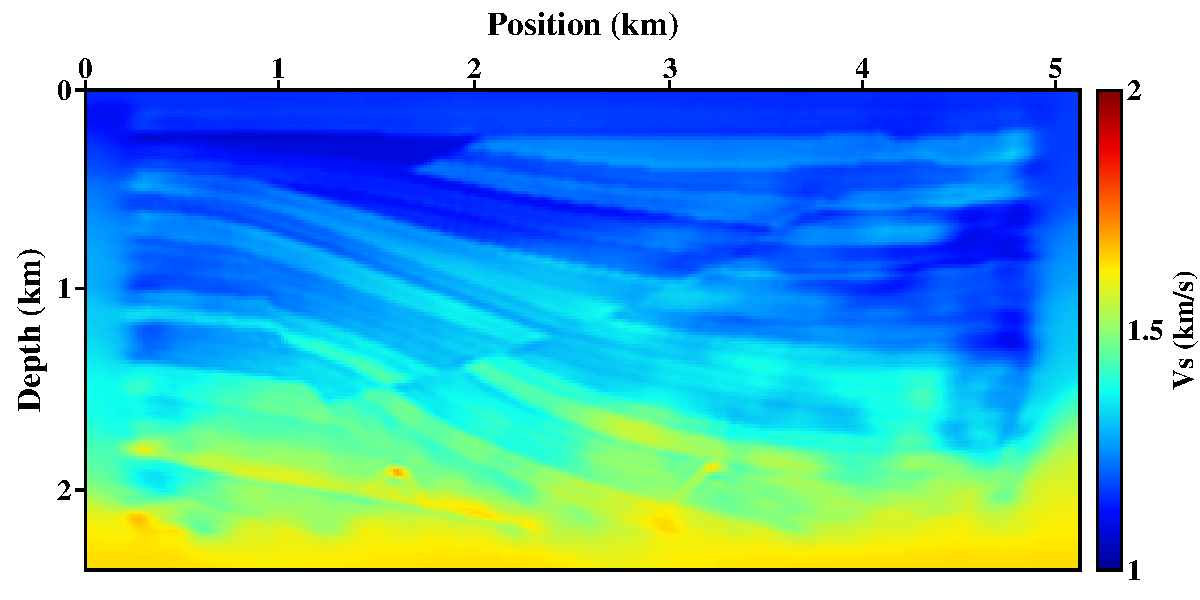
\includegraphics[width=0.5\textwidth]{sigbee2/Fig/nodevs.pdf}}
   \caption{
	   EFWI results using the ERTI model as starting model. (a) $V_p$, (b) $V_s$.
%	   Inverted results of WERTI and EFWI. (a) and (b) are inverted $V_p$ and
%       $V_s$ model through two-stage elastic WERTI with the linearly increased models
%       as initial models. (c) and (d) are inverted $V_p$ and $V_s$ through EFWI using
%   (a) and (b) as starting models.
   }
   \label{fig:EWERTI+EFWI}
\end{figure}
\begin{figure}[!htb]
   \centering
   \subfloat[]{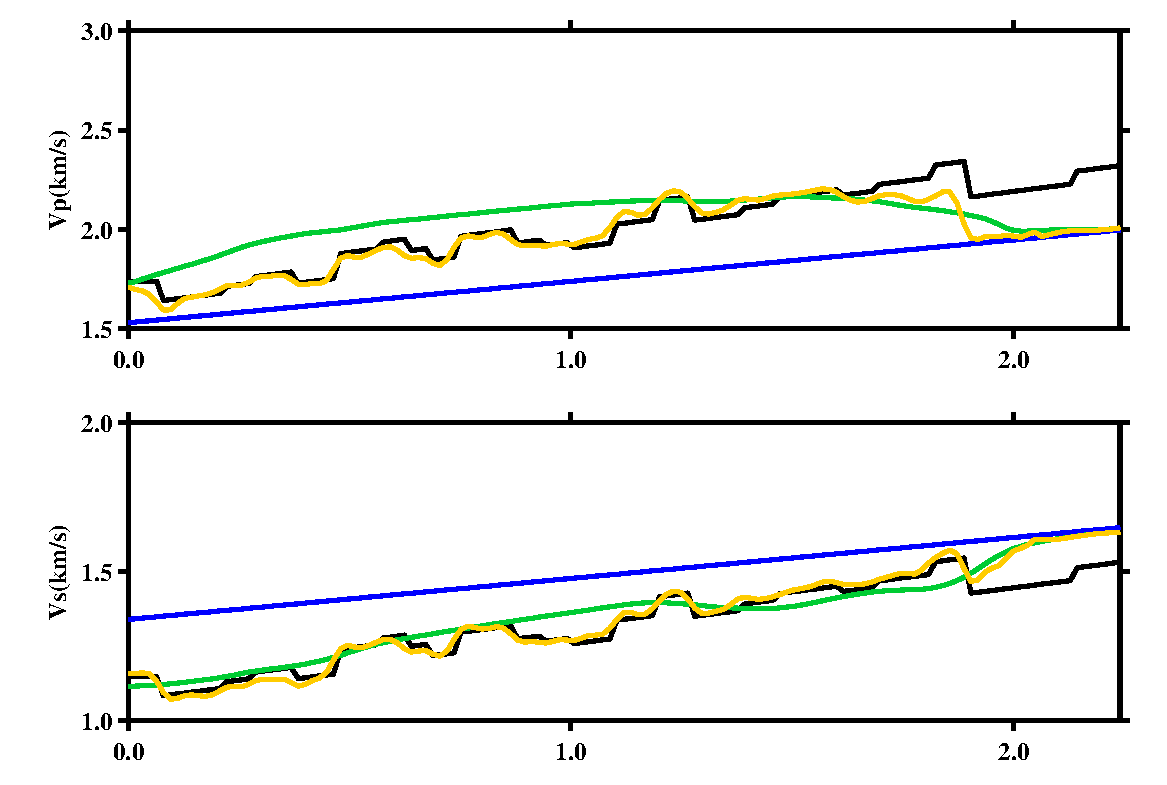
\includegraphics[width=0.5\textwidth]{sigbee2/Fig/1km.pdf}}
   \subfloat[]{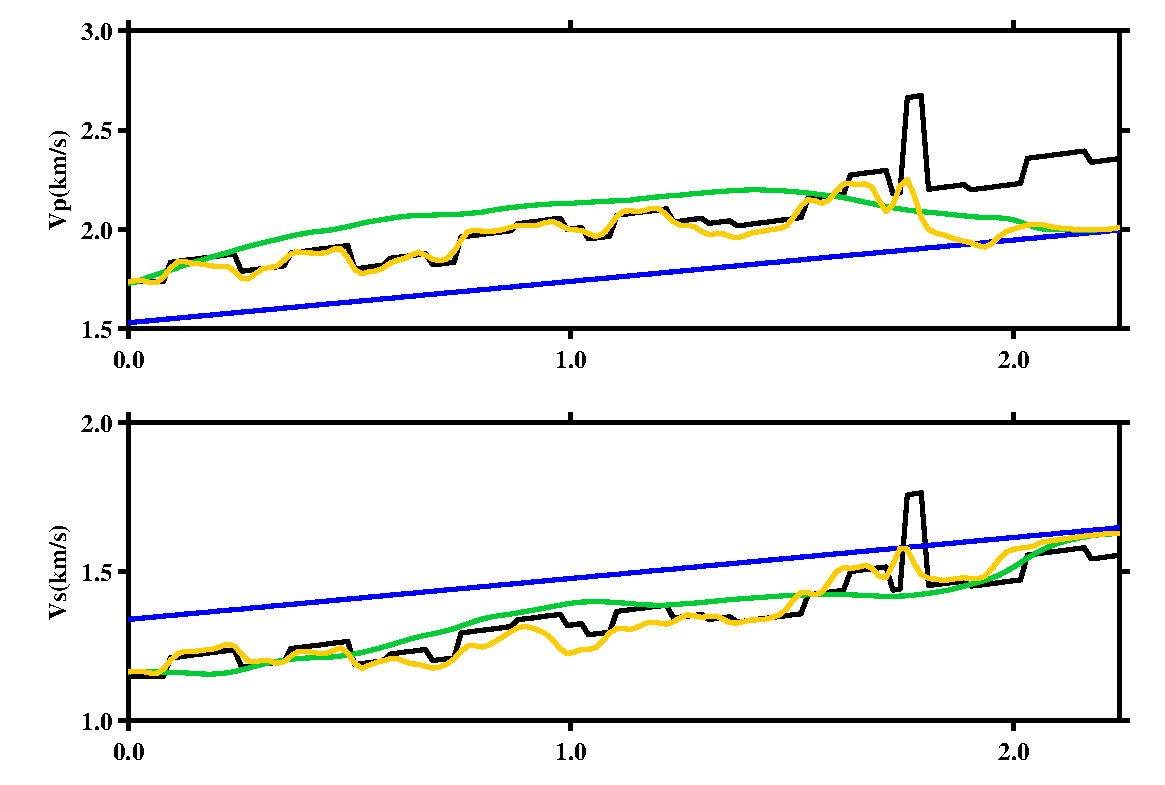
\includegraphics[width=0.5\textwidth]{sigbee2/Fig/3km.pdf}}
   \caption{
	   Vertical profile of ERTI and EFWI model at 1.4km (a) and 3km (b).
	   The black and blue lines denote the true and initial model. The green and yellow denote
	   the ERTI and EFWI model.
%	   Vertical profiles of elastic WERTI and EFWI results at 1.4km (a) and
%       3km (b). The black and blue lines indicate the true and linearly increased
%       initial model. The green and yellow lines indicate the WERTI and EFWI results,
%       respectively.
   }
   \label{fig:Profiles}
\end{figure}
\begin{figure}[!thb]
   \centering
   \subfloat[]{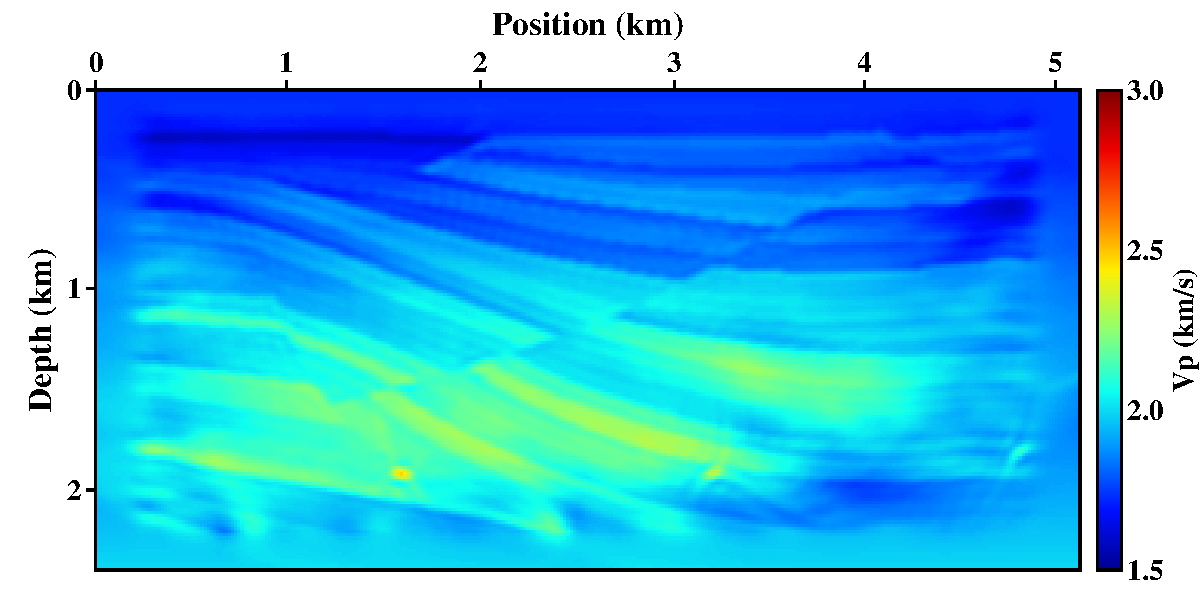
\includegraphics[width=0.5\textwidth]{sigbee2/3Hzvp.pdf}}
   \subfloat[]{\includegraphics[width=0.5\textwidth]{sigbee2/3Hzvs.pdf}}\\
   \subfloat[]{\includegraphics[width=0.5\textwidth]{sigbee2/5Hzvp.pdf}}
   \subfloat[]{\includegraphics[width=0.5\textwidth]{sigbee2/5Hzvs.pdf}}\\
   \subfloat[]{\includegraphics[width=0.5\textwidth]{sigbee2/7Hzvp.pdf}}
   \subfloat[]{\includegraphics[width=0.5\textwidth]{sigbee2/7Hzvs.pdf}}\\
   \caption{EFWI results with different starting frequency. (a), (c), (e) are $V_p$,
   (b), (d), (f) are $V_s$.
   The starting frequency are 3Hz, 5Hz and 7Hz from top to bottom row, respectively.
   }
   \label{fig:LowFreqCut_EFWI}
\end{figure}

\bibliographystyle{seg}
\bibliography{reference}
